\documentclass[a4paper]{jpconf}

% graphics packages
\usepackage{graphicx}
\usepackage{stackengine}
\usepackage{subfigure}
\usepackage{float}

% algorithm packages
%\usepackage{algpseudocode}
%\usepackage{algorithm}
\usepackage{amsmath}

% symbols
\usepackage{gensymb}

% reference packages
\usepackage{cleveref}
\usepackage{url}

% formatting packages
\usepackage{enumitem}

\graphicspath{{./final_images/}}

% editing packages
\usepackage{todonotes}

\begin{document}

\title{Reducing multi-modality in the wind farm layout optimization problem}

\author{J~J~Thomas, S~McOmber, and A~Ning}
\address{Department of Mechanical Engineering,
Brigham Young University, Provo, Utah, USA}
\ead{jaredthomas@byu.net}

\begin{abstract}
	This paper presents a process using an approach related to  continuation optimization methods for reducing multi-modality in the wind farm layout optimization problem, referred to as Wake Expansion Continuation (WEC). The reduction in multi-modality is achieved by starting with an increased wake spread, while maintaining normal velocity deficits at the center of the wakes, and then reducing the wake spread for each of a series of optimization runs until the standard wake spread is used. Two optimization cases were tested, one with 16 turbines and one with 38 turbines, by optimizing from 200 different starting positions with a gradient-based method, a gradient-free method, and a gradient-based method using WEC. Results using WEC show a $4\%$ mean optimized annual energy production (AEP) improvement compared to gradient-based optimization without WEC for both test cases. A gradient-free algorithm had a mean optimized AEP that was $1\%$ higher than WEC for the 16-turbine case, but WEC resulted in a $10\%$ higher mean optimized AEP compared to a gradient-free optimization method for the 38-turbine problem. These results are specific to the test cases and may not be generally representative.
\end{abstract}

\section{Introduction}
%The wind farm layout optimization (WFLO) problem 
%is studied extensively due to its potential to reduce the cost of wind energy significantly. However, the problem 
%
%has been determined to be of Non-Deterministic Polynomial Optimization (NPO) complete complexity, meaning that it 
%
%is extremely difficult to solve reliably \cite{acero2014}. The difficulty arises primarily from the large number of variables and constraints required for realistic problems and the multi-modal nature of the WFLO problem. This combination of issues is problematic for all optimization methods. The optimization methods used to solve the WFLO problem can be loosely grouped into two primary types: gradient-free methods and gradient-based methods. For the sake of brevity, we will discuss only gradient-based methods in this extended abstract.
%
%Gradient-free methods are the most used of the two methods. Gradient-free methods are fairly straight forward to use and can theoretically find global optima regardless of whether or not the problem is multi-modal. However, gradient-free methods have high computational costs when optimization problems have many variables, and so solution quality is compromised in practice by stopping the algorithm early \cite{rethore2014}.

The difficulty of solving the wind farm layout optimization (WFLO) problem is primarily due to the large number of variables and constraints required for realistic problems and the multi-modal nature of the problem's design space. Gradient-free optimization methods are the most common methods used to solve the WFLO problem. However, gradient-free methods have been shown to have reduced performance with high dimensional problems \cite{rios2013-grad-free-comparison}. The WFLO scales quickly to high dimensions as the number of turbines is increased. Gradient-based optimization methods are well suited for high dimensional problems. Gradient-based methods are not widely used for WFLO problems, but are gaining interest due to their relatively low computational cost and their ability to handle many variables and constraints. However, gradient-based methods are highly susceptible to local optima \cite{acero2014}. Despite this weakness, they have been shown to find good solutions to WFLO problems \cite{fleming2015, guirguis2016, gebraad2017-Maximization-Annual}.  

Many techniques have been presented to make the WFLO problem more tractable, including discretization, multi-start, and hybrid approaches. Discretization techniques, used with gradient-free methods, attempt to simplify the problem by reducing the number of possible solutions \cite{mosetti1994, grady2005}. Through discretization, the number of possible turbine locations within a wind farm can be reduced from infinite to something on the order of hundreds of locations. However, discretization disregards any locations that are not pre-selected, and can thus preclude this approach from finding even a local optimum. It is also possible that constraints on variables other than position may render the discretized optimization problem intractable. Multi-start approaches involve running many optimizations of one problem with different starting points \cite{gonzalez2014}. This approach reduces the sensitivity of gradient-based optimization methods to local optima. Hybrid approaches combine gradient-based and gradient-free algorithms iteratively \cite{rethore2014,graf2016, mittal2017}, 
%The idea is that the gradient-free method can be used until it seems to be converging on a solution, and then the output of the gradient-free algorithm can be used to warm start a gradient-based algorithm that can efficiently converge on the nearest optimum. 
%
and, depending on the problem size, can yield result quality comparable to multi-start approaches \cite{rethore2014}. While each of these techniques yield improved results, there is still need for improvement because current methods have a wide spread in the quality of results, are highly dependent on starting locations, and/or artificially limit the design space. These limitations indicate that the optimizations are not converging to the global optimum.

Current methods seek to avoid local optima by searching the existing design space more broadly. This approach becomes intractable for large optimization problems with many variables and constraints. To address this issue, we propose a process for use with gradient-based optimization algorithms that temporarily reduces the number and magnitude of local optima using an approach related to continuation optimization methods such as the approach given in \cite{mobahi2015}. However, while continuation optimization uses a numerical approximation of the design space, our proposed process takes advantages of the physical properties of the design space directly. We will refer to the new process as Wake Expansion Continuation, or WEC.

\section{Wake Expansion Continuation}\label{sec:dsrop}
The two primary characteristics that simple wake models seek to capture are wake spread and velocity deficit. These characteristics in turn largely determine the shape of the wind farm layout design space. The fluctuations of wind speed as turbines move in and out of the wakes during optimization are primarily responsible for the multi-modal nature of the WFLO problem. 

During optimization, the spaces between wakes translate to locally optimal locations for turbines. However, it is often the case that there are more optimal turbine locations that are not found by the optimizer because the turbines are effectively stuck on the peaks between wakes. The proposed WEC seeks to overcome this problem by temporarily reducing the multi-modality of the design space. The WEC is comprised of three basic steps:
\begin{enumerate}[label=\arabic*)]
	\item Determine how the wake spread and wake deficit are controlled for the selected model(s).
    \item If necessary, add a factor to the model such that the wake spread can be directly controlled without significantly altering the wake deficit in the center of the wake. (While we assume that it is important to avoid altering the velocity in the wake significantly, this assumption should be the subject of future study.)
    \item Run a series of optimizations such that the wake spread is larger than normal for the first optimization, and then reduces with each subsequent optimization until the wake spread is no longer altered from the original model. The result of each optimization after the first should be started using the optimal layout found in the previous optimization.
\end{enumerate}
By spreading the wakes, we can effectively fill in the gaps between wakes so that a gradient-based optimization algorithm can bypass local optima and proceed to a better solution. Another way of think about this is that by spreading the wakes, more turbines see the influence of each wake, which provides more information to the gradient-based optimization algorithm about the design space through the Jacobian.

Because of the general nature of the proposed method, it could theoretically be applied to a range of wake models. In this study we have applied WEC to the cosine version of the Jensen model \cite{jensen1983}, the FLORIS model \cite{gebraad2014,thomas2017-Improving-FLORIS}, and the 2016 version of the Bastankhah and Port\'e-Agel wake model \cite{bastankhah2016}.

\section{Wake and Wind Farm Models}
\subsection{The Jensen Cosine Wake Model}
The Jensen Cosine wake model is used to calculate the velocity deficit of the wind at any distance downwind from the waking turbine. The author, N. O. Jensen, derived the equation from a momentum balance of the air passing through a wind turbine. The equation for the Jensen Cosine wake model is displayed below in \cref{eq:JensenVelocityDeficit}.

% Equation for the Jensen Cosine velocity deficit.
\begin{equation}
    \frac{\Delta \bar{u}}{\bar{u}_\infty} = 1 - 2a \bigg(\frac{f_\theta r_0}{r_0 + \alpha x} \bigg)^2
    \label{eq:JensenVelocityDeficit}
\end{equation}

In \cref{eq:JensenVelocityDeficit}, $V$ represents the wind velocity at any distance $x$ downstream of the waking turbine, $U$ represents the free-stream wind velocity, $f_\theta$ represents the cosine factor (see \cref{eq:JensenCosineAdjustment}), $r_0$ represents the radius of the wind turbine, and $a$ represents the axial induction (ideal value of $a = 1/3$).

\subsection{The FLORIS Wake Model}
The FLORIS wake model was developed by Gebraad et al. based on the Jensen-Cosine wake model \cite{Gebraad2014}. It is similar to the Jensen-Cosine model in that the velocity deficit is constant within certain regions of the wake; however, whereas the Jensen-Cosine model describes turbines as having a single velocity for the whole cross-section of the wake, the FLORIS model describes turbine wakes as having three separate wake zones, each with a different velocity deficit (see \cref{fig:FLORISDiagram}) \cite{Gebraad2014}. The FLORIS wake model contains many parameters that are tuned based on datasets produced by Large-Eddy Simulations (LES) run on the Simulator for Off/Onshore Wind Farm Applications (SOWFA) \cite{Fleming2015}. For this comparison study, we used the FLORIS model after it had been tuned to the National Renewable Energy Laboratories (NREL) 5-MW wind turbine.

\subsection{The Bastankhah and Port\'e-Agel Wake Model}
In the Bastankhah and Port\'e-Agel wake model, the two primary characteristics of the wakes, wake deficit and wake spread, are particularly easy to differentiate. This, along with the smoothness and differentiability of the model, make it a good example for demonstrating WEC. We used the Bastankhah and Port\'e-Agel wake model, as defined in \cref{eq:bpa} \cite{bastankhah2016}, along with part of the Niayifar and Port\'e-Agel wind farm model \cite{niayifar2016}. 
%
\begin{equation}
	\frac{\Delta \bar{u}}{\bar{u}_{\infty}} = \Bigg(1-\sqrt{1-\frac{C_T \cos{\gamma}}{8 \sigma_y \sigma_z/d^2}}~\Bigg) \exp{\bigg(-0.5\Big(\frac{y-\delta}{\sigma_y}\Big)^2\bigg)}\exp{\bigg(-0.5\Big(\frac{z-z_h}{\sigma_z}\Big)^2\bigg)}
	 \label{eq:bpa}
\end{equation}
%
Where $\Delta \bar{u} / \bar{u}_{\infty}$ is the wake velocity deficit, $C_T$ is the thrust coefficient, $\gamma$ is the upstream turbine's yaw angle with respect to the inflow direction, $y-\delta$ and $z-z_h$ are the distances of the point of interest from the wake center in the cross-stream horizontal and vertical directions respectively, and $\sigma_y$ and $\sigma_z$ are the standard deviations of the wake deficit in the cross-stream horizontal and vertical directions as defined in \cref{eq:sigmay,eq:sigmaz}.
%
\begin{equation}\label{eq:sigmay}
	\sigma_y = k_y (x - x_0) + \frac{D_r \cos{\gamma}}{\sqrt{8}}
\end{equation}
%
\begin{equation}\label{eq:sigmaz}
	\sigma_z = k_z (x - x_0) + \frac{D_r}{\sqrt{8}}
\end{equation}
%
In \cref{eq:sigmay,eq:sigmaz}, x is the downstream distance from the turbine generating the wake to the point of interest, $x_0$ is the length of the wake potential core, $D_r$ is the diameter of the turbine generating the wake, and $k_y$ and $k_z$ were determined as a function of turbulence intensity ($I$) as defined in \cref{eq:kstar}\cite{niayifar2016}.
%
\begin{equation}\label{eq:kstar}
	k^* = 0.3837I + 0.003678
\end{equation}
%
While the Niayifar and Port\'e-Agel wind farm model calculates $k^*$ based on local turbulence intensity at each turbine, the local turbulence intensity calculations introduce more local optima and discontinuities. For this reason, we chose to ignore local turbulence intensity in this study. While local turbulence intensity does impact the accuracy of the power predictions, it does not alter the general trends within the design space, and most simple wake models ignore local turbulence intensity. We are currently investigating possible solutions to the problems with the local turbulence intensity calculations.
%
%
% We used the Bastankhah and Port\'e-Agel wake model in this study, as defined in \cref{eq:bpa} \cite{bastankhah2016}
% \begin{equation}
% 	\frac{\Delta \bar{u}}{\bar{u}_{\infty}} = \Bigg(1-\sqrt{1-\frac{C_T \cos{\gamma}}{8 \sigma_y \sigma_z/d^2}}~\Bigg) \exp{\bigg(-0.5\Big(\frac{y-\delta}{\sigma_y}\Big)^2\bigg)}\exp{\bigg(-0.5\Big(\frac{z-z_h}{\sigma_z}\Big)^2\bigg)}
% 	 \label{eq:bpa}
% \end{equation}
% %
% Where $\Delta \bar{u} / \bar{u}_{\infty}$ is the wake velocity deficit, $C_T$ is the thrust coefficient, $\gamma$ is the upstream turbine's yaw angle with respect to the inflow direction, $\sigma_y$ and $\sigma_z$ are the standard deviations of the wake in the cross-stream and vertical directions respectively, and $y-\delta$ and $z-z_h$ are the distances of the point of interest from the wake center in the cross-stream and vertical directions respectively. For more details on the Bastankhah and Port\'e-Agel wake model, see reference \cite{bastankhah2016}.
%%
%Where 
%%
%\begin{equation}
%	\sigma_y = k_y (x - x_0) + \frac{D_r \cos{\gamma}}{\sqrt{8}}
%	\label{eq:sigmay}
%\end{equation}
%%
%%
%\begin{equation}\label{eq:sigmaz}
%	\sigma_z = k_z (x - x_0) + \frac{D_r}{\sqrt{8}}
%\end{equation}
%%
%and
%%
%\begin{equation}
%	\frac{x_0}{D_r} = \frac{\cos{\gamma }(1+\sqrt{1-C_T})}{\sqrt{2} (\alpha ^* I + \beta ^* (1- \sqrt{1-C_T}))}
%\end{equation}

The Gaussian shape of the Bastankhah and Port\'e-Agel wake model is well suited for gradient-based optimization because it is smooth, continuous, and has no flat regions. However, in the near wake, the model can either be flat, which can cause premature convergence, or be undefined, which can cause optimizations to fail. To resolve this issue, we used a simple solution for optimization purposes only: a linear interpolation of the velocity deficit, from the rotor hub to the length of the wake potential core, that maintains the Gaussian shape of the wake all the way to the rotor location. Because no turbines will be placed in this region of the wake in the final optimized layout, the accuracy of the model in the near wake is second in importance to wake shape and continuity. 

\subsection{Power Model}
We combined the wake deficits using a linear combination method as discussed in \cite{niayifar2016}. To save computation time, the inflow wind speed at each turbine was approximated using a single sample at the wind turbine hub location. Individual turbine inflow wind velocities, $U_i$, were solved consecutively from upstream to downstream. The power output of each turbine was then calculated based on \cref{eq:power}
%
\begin{equation}\label{eq:power}
P_i = \frac{1}{2}\rho A_{r,i}C_P U_i^3
\end{equation}
%
where $\rho$ is the air density, $A_{r,i}$ is the rotor-swept area of turbine $i$, and $C_P$ is the power coefficient. The values of $C_P$ and $C_T$ were determined based on the calculated inflow velocity of each turbine and the power curve and thrust coefficient curve presented in \cite{niayifar2016}.

\section{Applying WEC to the Jensen Cosine Wake Model}
In this section we apply WEC, step by step, as presented in \cref{sec:dsrop} to the Jensen Cosine wake model.  

%Just as the Bastankah and Port\'e-Agel model could be adjusted with a relaxation factor ($\xi$) \cite{Thomas2018}, so may the Jensen-Cosine model. In the BPA wake model, the relaxation factor was applied to the terms describing the turbine's wake width, thereby expanding the wake's width without affecting the rate of wake spread. In a similar manner, the relaxation factor was applied to the radius of the wake width in the Jensen-Cosine model (\cref{eq:JensenWECWakeWidth}).

\subsection{Jensen Cosine WEC Step (1)}
\todo{Spencer}
%Identify where the magnitude and spread of the wake are within the Jensen Cosine equation.

The cosine factor, $f_\theta$, in \cref{eq:JensenVelocityDeficit} controls the wake spread for the Jensen Cosine wake model. By breaking down the cosine factor into its constituent parameters, it is possible to adjust the wake spread without affecting the velocity deficit in the center of the wake.

\subsection{Jensen Cosine WEC Step (2)}
\todo{Spencer}
%Apply relaxation factor to the Jensen Cosine equation. Show the aep vs crosswind position plot to demonstrate the velocity deficit is unchanged in the center of the wake and that the wakes are capable of being spread out. Briefly describe this plot and how the wec factor affects it.

This section will break down how the cosine factor, $f_\theta$, is determined, and how a relaxation factor may be applied to spread the wake without impacting the velocity deficit of the wake's center. A figure displaying the relevant parameters is displayed below in \cref{fig:JensenDiagrams}, and an equation describing the cosine factor may be seen below in \cref{eq:JensenCosineAdjustment}.

% Diagrams showing wake described by Jensen Cosine model.
\begin{figure}[h]
    \centering
    \subfigure[]{
        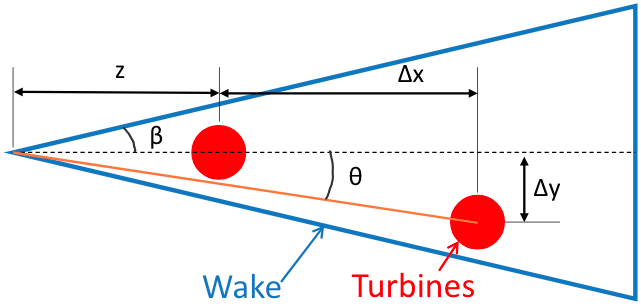
\includegraphics[width=0.4\textwidth, trim={0cm 0cm 0cm 0cm}]{JensenDiagram1}
    }
    \subfigure[]{
        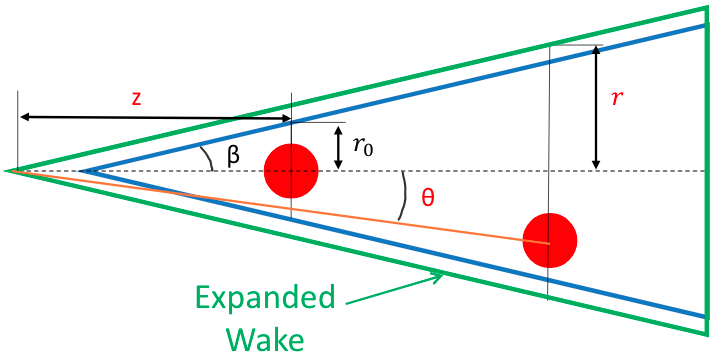
\includegraphics[width=0.4\textwidth, trim={0cm 0cm 0cm 0cm}]{JensenDiagram2}
    }
    \caption{Diagrams describing the overhead geometry of the Jensen Cosine turbine wake model. Two sub-figures are required to more clearly display all the relevant wind farm parameters. It is assumed the wind is blowing to the right in these figures. The wake's "fulcrum" is represented as the left-most vertex of the wake within each subfigure. The dashed line down the middle represents the center line of the wake.}
    \label{fig:JensenDiagrams}
\end{figure}

% Enter the Cosine Adjustment Equation to Jensen's Wake Model.
\begin{equation}
    f_\theta = \frac{1 + cos(n\theta)}{2}
    \label{eq:JensenCosineAdjustment}
\end{equation}

In \cref{eq:JensenCosineAdjustment}, $n$ represents an adjustment factor based upon the boundary angle of the wake spread, $\beta$, as shown in \cref{fig:JensenDiagrams}. This boundary angle has a default value of $\beta = 20 \degree$. The value for $n$ can be calculated below in \cref{eq:nFactor}, where $\beta$ is in units of radians.

% Equation to determine the factor n in the Jensen Cosine factor.
\begin{equation}
    n = \pi / \beta
    \label{eq:nFactor}
\end{equation}

As can be seen in \cref{eq:JensenCosineAdjustment}, $f_\theta$ is a function of $\theta$, which represents the angle between the wake's center line, the wake's fulcrum, and the downwind turbine's location. This angle $\theta$ can be determined using \cref{eq:Theta}, which was obtained from \cref{fig:JensenDiagrams} through trigonometry.

% Equation for calculating theta, the angle between the wake's fulcrum and the wake-receiving turbine.
\begin{equation}
    \theta = \tan^{-1}\Big( \frac{\Delta y}{\Delta x + z} \Big)
    \label{eq:Theta}
\end{equation}

In \cref{eq:Theta}, $\Delta x$ and $\Delta y$ represent the spacing between the upwind turbine and the downwind turbine with respect to the $x$ and $y$ coordinate frames, respectively. The variable $z$ represents the distance between the wake's fulcrum and the upwind turbine (see \cref{fig:JensenDiagrams} for a visual representation of these spacing variables). By adjusting the value of $z$, we are able to increase or decrease the wake's spread. An expression for $z$ can be found below in \cref{eq:FulcrumDistance}, which was determined from \cref{fig:JensenDiagrams} using trigonometry.

\begin{equation}
    z = \frac{r}{tan(\beta)}
    \label{eq:FulcrumDistance}
\end{equation}

In \cref{eq:FulcrumDistance}, $r$ represents the radius of the wake at any point $x$ downwind of the upwind turbine. This is where the wake spread may be directly adjusted by applying a relaxation factor, as seen below in \cref{eq:JensenWECWakeWidth}.

% Enter the equation where the relaxation factor is being inserted into the Jensen Cosine model.
\begin{equation}
    r = \xi r_0
    \label{eq:JensenWECWakeWidth}
\end{equation}

In \cref{eq:JensenWECWakeWidth}, $\xi$ represents the relaxation factor from WEC, and $r_0$ represents the rotor radius, and $r$ represents the radius of the wake at the wind turbine. As seen in the above equation, the radius of the wake may be directly scaled by the relaxation factor from WEC.

The relaxation factor, $\xi$, may be propagated back into the original Jensen Cosine equation, \cref{eq:JensenVelocityDeficit}. By substituting \cref{eq:JensenWECWakeWidth} into \cref{eq:FulcrumDistance}, we obtain \cref{eq:WECFulcrumDistance}, a representation of the new fulcrum distance as adjusted by the relaxation factor, $\xi$.

\begin{equation}
    z = \frac{\xi r_0}{tan(\beta)}
    \label{eq:WECFulcrumDistance}
\end{equation}

This new fulcrum distance, \cref{eq:WECFulcrumDistance}, may be substituted into \cref{eq:Theta} to obtain \cref{eq:ThetaWithFulcrumDist} below.

% Insert equation: sub z equation into theta equation.
\begin{equation}
    \theta = \tan^{-1}\Bigg( \frac{\Delta y}{\Delta x + \frac{\xi r_0}{tan(\beta)}} \Bigg)
    \label{eq:ThetaWithFulcrumDist}
\end{equation}

This new equation for $\theta$, \cref{eq:ThetaWithFulcrumDist}, may be substituted into \cref{eq:JensenCosineAdjustment} to obtain \cref{eq:JensenCosineAdjustmentWithThetaAndNFactor}, the cosine factor adjusted by WEC.

% Insert equation: sub n and theta into cosine factor.
\begin{equation}
    f_\theta = \frac{1}{2} \Bigg( 1 + cos \Bigg[ \frac{\pi}{\beta} \tan^{-1}\Bigg( \frac{\Delta y}{\Delta x + \frac{\xi r_0}{tan(\beta)}} \Bigg) \Bigg] \Bigg)
    \label{eq:JensenCosineAdjustmentWithThetaAndNFactor}
\end{equation}

Finally, by substituting \cref{eq:JensenCosineAdjustmentWithThetaAndNFactor} into \cref{eq:JensenVelocityDeficit}, we obtain the final equation for calculating the velocity deficit with the Jensen Cosine model (\cref{eq:JensenVelocityDeficitCombined}).

% Insert equation: final equation displaying the direct relationship between the velocity deficit and the relaxation factor, xi.
\begin{equation}
    \frac{\Delta \bar{u}}{\bar{u}_\infty} = 1 - 2a \Bigg[ \frac{1}{2} \Bigg(1 + cos\Bigg[\frac{\pi}{\beta} tan^{-1}\Bigg(\frac{\Delta y}{\Delta x + \frac{\xi r_0}{tan(\beta)}} \Bigg) \Bigg] \Bigg) \bigg(\frac{r_0}{r_0 + \alpha x} \bigg) \Bigg]^2
    \label{eq:JensenVelocityDeficitCombined}
\end{equation}

Because we have inserted the relaxation factor, $\xi$, into \cref{eq:JensenVelocityDeficitCombined}, we may adjust the wake spread without changing the velocity deficit in the center of the wake. Note that this is true because when $\Delta y = 0$, the term inside the inverse tangent in \cref{eq:JensenVelocityDeficitCombined} goes to zero, regardless of the value of $\xi$. Because this is the only place where the relaxation factor is found in \cref{eq:JensenVelocityDeficitCombined}, this means that the velocity deficit will be constant with respect to $\xi$ at the wake center. Figure (\cref{fig:smoothing_locations_Jensen,fig:JensenLocalOptSmoothed}) below confirms this prediction and confirms that local optima can be smoothed out through WEC for the Jensen Cosine model.

% Figure describing setup for aep vs crosswind position tests for Jensen
\begin{figure}[ht]
	\centering
	\begin{minipage}[t]{0.43\textwidth}
		\centering
		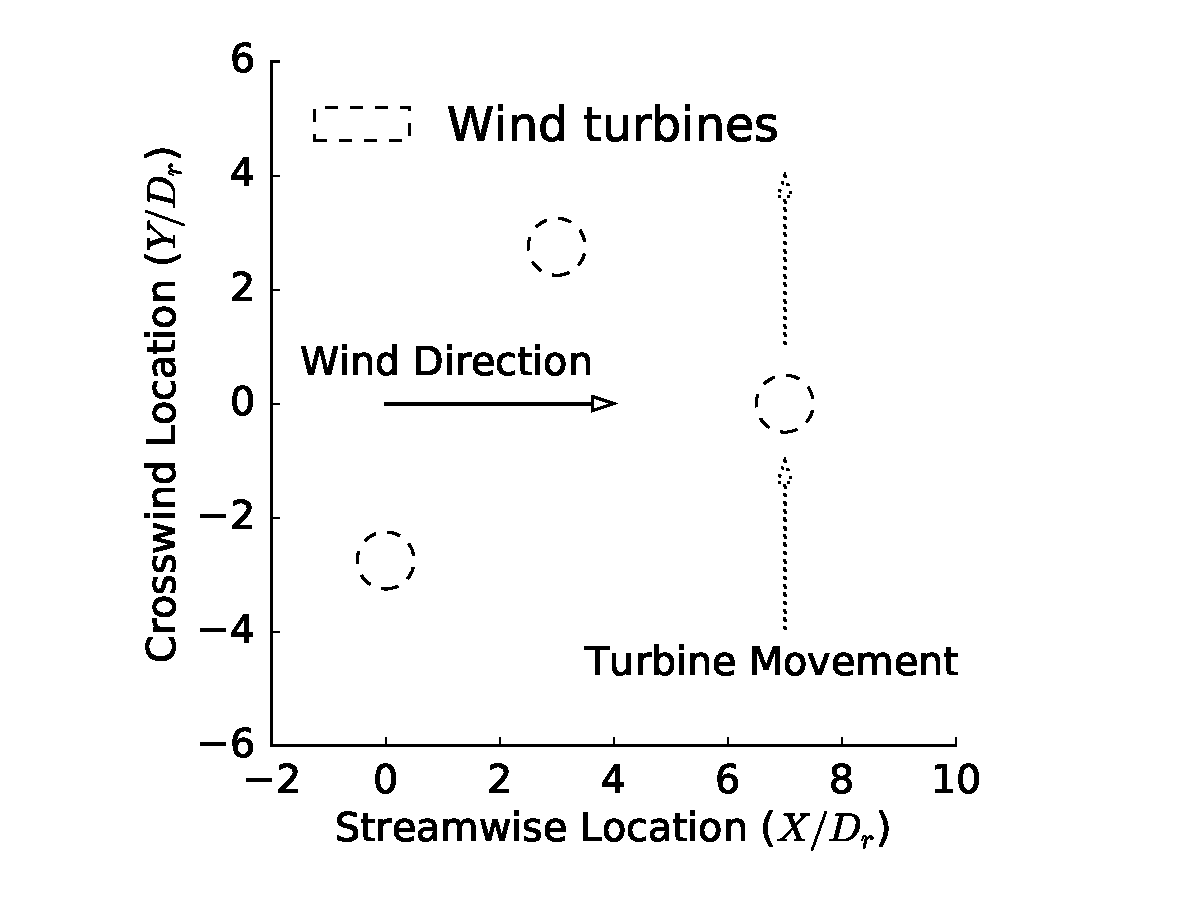
\includegraphics[width=\textwidth, trim={2cm 0cm 2cm 0cm}, clip]{smoothing_locations}
		\caption{Simple design space used to demonstrate the effects of the relaxation factor, $\xi$, on the wind farm layout design space (see \cref{fig:smoothing_visualization}).}
		\label{fig:smoothing_locations_Jensen}
	\end{minipage}\hspace{1pc}
% Figure displaying results from aep vs crosswind position tests for Jensen
	\begin{minipage}[t]{0.52\textwidth}
		\centering
		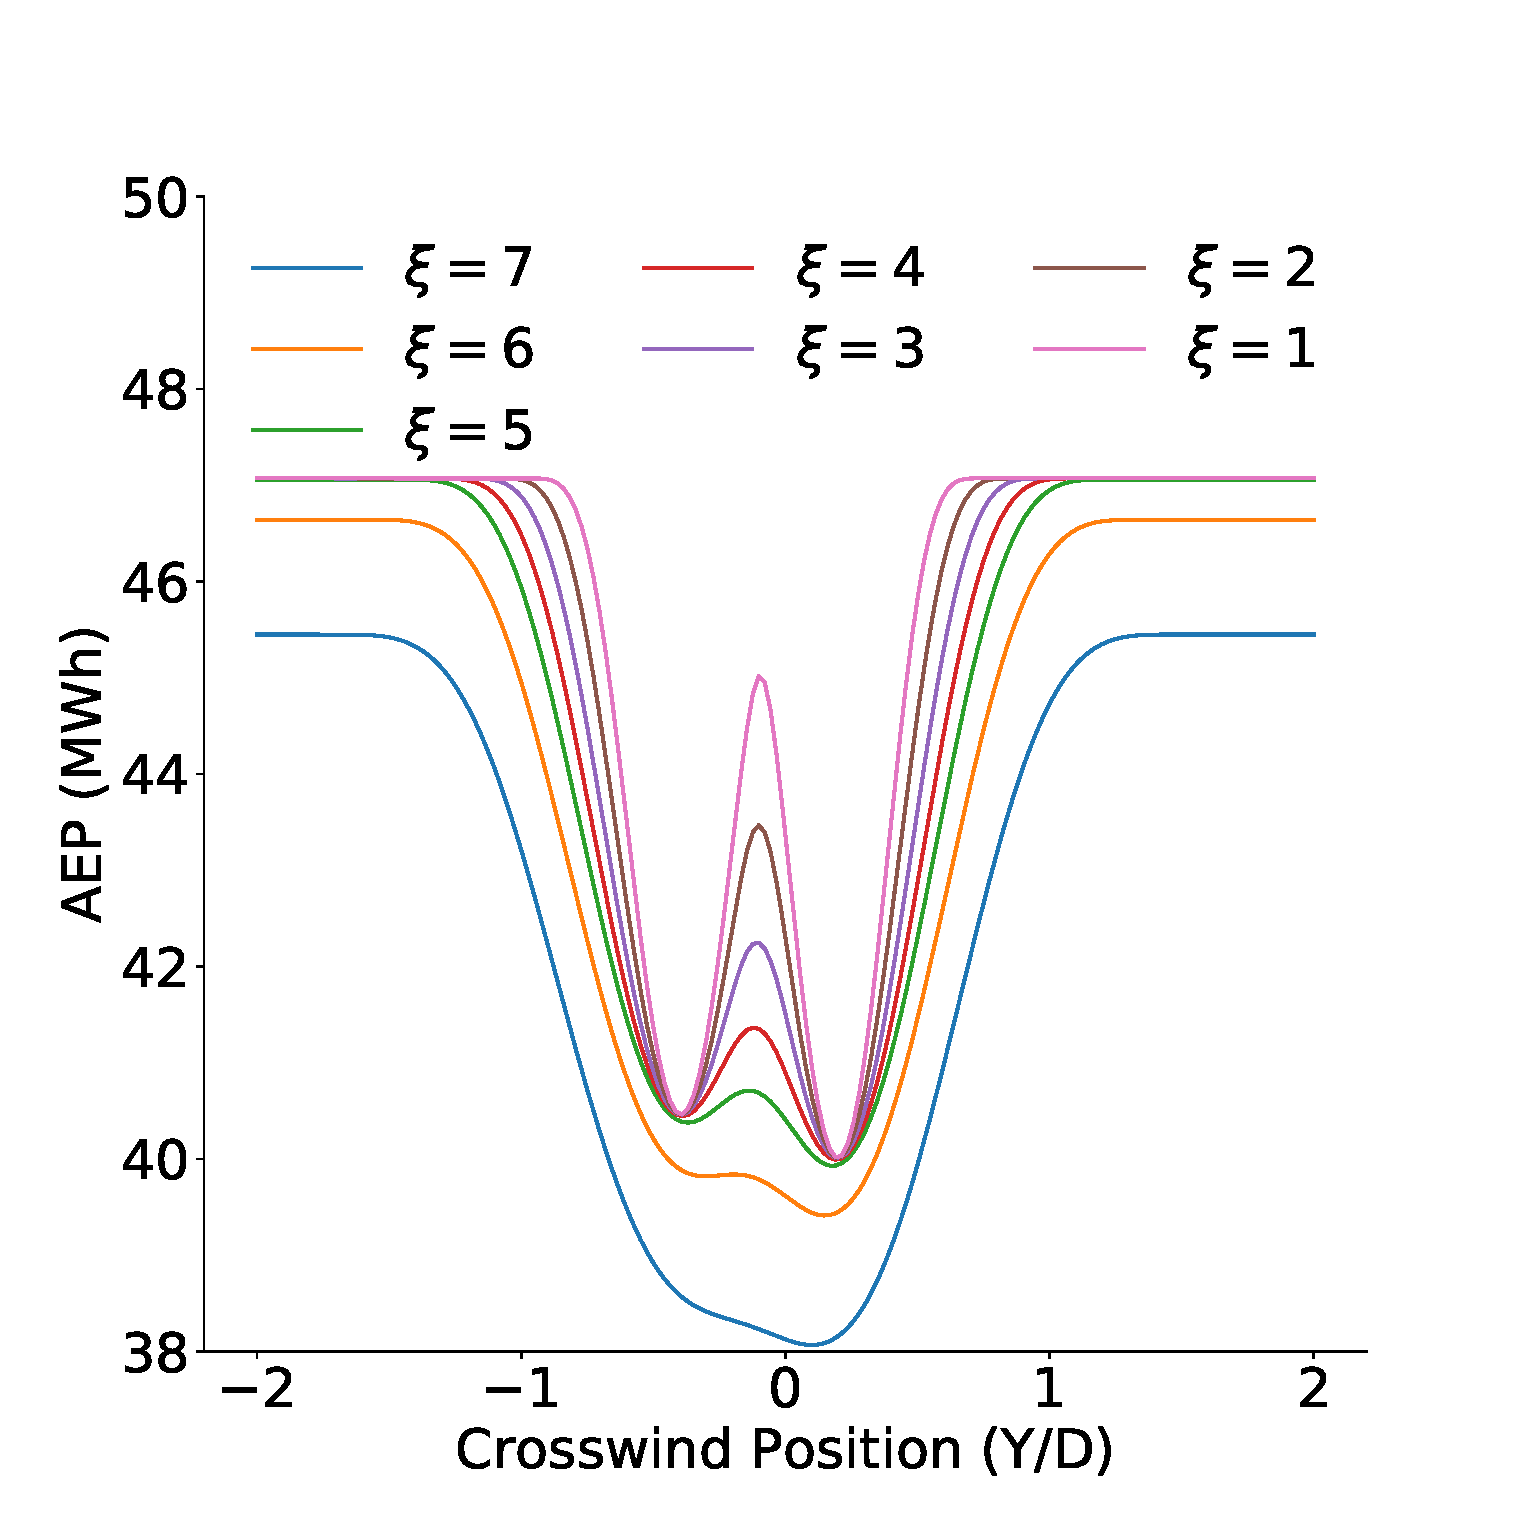
\includegraphics[width=\textwidth]{JensenWECMultipleTurbinesAEP}
		\caption{AEP plotted against crosswind position of the turbine seen in \cref{fig:smoothing_locations_Jensen}. Drops in AEP occur where wakes are present. Note the local optimum between the two wakes that is smoothed out as the WEC factor increases.}
		\label{fig:JensenLocalOptSmoothed}
	\end{minipage}
\end{figure}

\subsection{Jensen Cosine WEC Step (3)}
\todo{Spencer}
%Describe how the optimization would actually use WEC (e.g., multiple wec factors decreasing from some value to 1, at which point the model is normal again. Warm start new optimizations with previous optimization's results). Report which values for wec factor were used.

The optimization for the Jensen Cosine model with WEC is simple in concept. A reasonably large relaxation factor is chosen for the first optimization, which results in an optimized wind farm layout where all local optima have been smoothed out. A new, lower relaxation factor is chosen, and the results from the previous optimization are used as a warm start for the new optimization. This process repeats until the relaxation factor is equal to one, at which point the optimization being solved is identical to optimizing the original Jensen Cosine model without WEC. In this way, WEC allows the optimization to escape local optima in the first few optimizations, but the Jensen Cosine model becomes more accurate as the relaxation factor is decreased closer to one. Through trial and error, we decided to use the following relaxation factors: $\xi = [3, 2.75, 2.5, 2.25, 2, 1.75, 1.5, 1.25, 1, 1]$. The selection of relaxation factors should be the topic of future research.

\section{Applying WEC to the FLORIS Wake Model}
In this section we apply WEC, step by step, as presented in \cref{sec:dsrop} to the FLORIS wake model.  

%\todo{need to get better figure. remember to update caption once new figure inserted.}
%\begin{figure}[h]
%    \centering
%    \includegraphics[width=0.3\linewidth]{FLORISDiagram1}
%    \caption{Diagram displaying the three wake zones in the FLORIS turbine wake model. A higher quality diagram would have been constructed if there had been sufficient time. The black outer lines represent the outermost wake zone (mixing zone) which expands from the wind turbine as the air travels downstream. The blue lines represent the middle wake zone (far zone) which retains nearly the same width with distance from the turbine. Finally, the green lines represent the innermost wake zone (near wake) which converges to a point some distance from the turbine. The velocity deficit associated with each wake zone increases from the outermost wake zone to the innermost wake zone.}
%    \label{fig:FLORISDiagram}
%\end{figure}

We began by determining where in the FLORIS wake model to apply the relaxation factor. Similar to the Jensen-Cosine wake model, we decided to apply the relaxation factor to the original wake diameter in the FLORIS wake model. Because the increased wakes would result in larger wake overlaps, we decided that our implementation of WEC would need to occur before any area overlap calculations took place. Based on Figure 3 of Gebraad et. al's paper \cite{Gebraad2014}, we decided that the most intuitive option would be to implement the relaxation factor in the wake diameter equation (\cref{eq:FLORISWakeWidth}).

\begin{equation}
    D_{w,i,q} = D_i + 2k_em_{e,q}(x - X_i)
    \label{eq:FLORISWakeWidth}
\end{equation}

In \cref{eq:FLORISWakeWidth}, $D_{w,i,q}$ represents the diameter of the wake for the turbine of index $i$ within the wake-zone $q$, $D_i$ represents the rotor-diameter of turbine $i$, $k_e$ and $m_{e,q}$ represent wake expansion coefficients, $x$ represents the distance downwind from the wake-generating turbine to turbine $i$, and $X_i$ represents the x-coordinate of turbine $i$. In this equation, $k_e$ and $m_{e,q}$ determine the rate of expansion while $D_i$ represents an initial wake width. If we applied the relaxation factor to $k_e$ or $m_{e,q}$, the rate of wake expansion would be affected, which violates the conditions for WEC described at the start of the Methods section. On the other hand, applying the relaxation factor to $D_i$ would expand the wake without affecting the rate of wake expansion. Therefore, we decided to apply the relaxation factor to $D_i$ to obtain \cref{eq:FLORISWECWakeWidth}.

\begin{equation}
    D_{w,i,q}' = D_i' + 2k_em_{e,q}(x - X_i)
    \label{eq:FLORISWECWakeWidth}
\end{equation}

Where $D_{w,i,q}'$ represents the adjusted wake width from applying WEC and $D_i'$ represents the adjusted initial wake diameter from applying WEC. An equation for the adjusted initial wake diameter is seen below in \cref{eq:FLORISWECWakeDiameter}.

\begin{equation}
    D_i' = \xi D_i
    \label{eq:FLORISWECWakeDiameter}
\end{equation}

% Initial results from applying the above equations prompted us to adjust our methods. First, we decided to implement a cosine factor to smooth the results, as done by Thomas and Ning in \cite{Thomas2017}. Second, we noticed that the preliminary results from FLORIS indicated that the velocity deficit in the wake's center was not constant for all values of $\xi$. We determined that the cause of this error was the increase in wake width of the innermost wake-zone. By increasing this wake diameter, we were allowing the innermost wake-zone to propagate much farther downwind than it would without a relaxation factor. Thus, turbines near the center of the wake would experience the effects of the innermost wake-zone for high values of $\xi$ but not for lower values of $\xi$. This caused the velocity deficit in the center of the wake to differ with $\xi$.

% Originally, we resolved this issue by only applying the WEC relaxation factor to the middle and outermost wake zones. By doing so, we kept the innermost zone from propagating too far downstream and thereby ensured that the velocity deficit at the wake-center would be the same for all $\xi$. After more testing, however, we determined that failing to apply the relaxation factor to the innermost wake zone actually promoted the creation of a local optimum between two upwind turbines, which defeats WEC's purpose in smoothing out local optima. While the velocity deficit in the center of the wake is not preserved as well when applying WEC to the innermost wake zone, FLORIS performs better with WEC as a result of this change.

We applied \cref{eq:FLORISWECWakeWidth} to all wake zones within the FLORIS wake model. The resulting equations controlling the wake diameters for various wake zones in the FLORIS model are displayed below in \cref{eq:FLORISWECWakeDiameterPiecewise}. In this equation, $q$ represents the wake zone being used (i.e., $q = 1$ for the innermost wake zone, $q = 2$ for the middle wake zone, and $q = 3$ for the outermost wake zone).

\begin{equation}
    D_{w, i, q}' = \begin{cases}
        \xi D_i + 2k_em_{e, q} (x - X_i), & q = 1 \\
        \xi D_i + 2k_em_{e, q} (x - X_i), & q = 2 \\
        \xi D_i + 2k_em_{e, q} (x - X_i), & q = 3
    \end{cases}
    \label{eq:FLORISWECWakeDiameterPiecewise}
\end{equation}

\subsection{FLORIS WEC Step (1)}
\todo{Spencer}
Identify where the magnitude and spread of the wake are within the FLORISSE equation.

After searching through 

\subsection{FLORIS WEC Step (2)}
\todo{Spencer}
Apply relaxation factor to the FLORIS equation. Show the aep vs crosswind position plot to demonstrate the velocity deficit is unchanged in the center of the wake and that the wakes are capable of being spread out. Briefly describe this plot and how the wec factor affects it.

\subsection{FLORIS WEC Step (3)}
\todo{Spencer}
Describe how the optimization would actually use WEC (e.g., multiple wec factors decreasing from some value to 1, at which point the model is normal again. Warm start new optimizations with previous optimization's results). Report which values for wec factor were used.

\section{Applying WEC to the Bastankhah and Port\'e-Agel Wake Model}
In this section we apply WEC, step by step, as presented in \cref{sec:dsrop} to the Bastankhah and Port\'e-Agel wake model.  

\subsection{Bastankhah and Port\'e-Agel WEC Step (1)}
The first parenthetical term of \cref{eq:bpa} defines the magnitude of the velocity deficit. The exponential terms determine the wake spread. The wake spread and velocity deficit are coupled through $\sigma_y$ and $\sigma_z$. However, because the spread and magnitude are expressed in separate terms, it is possible to adjust one without impacting the other. 

\subsection{Bastankhah and Port\'e-Agel WEC Step (2)}
We gained independent control of the wake spread from the wake velocity deficit by applying a factor, $\xi$, to $\sigma_y$ and $\sigma_z$ inside the exponential terms of \cref{eq:bpa}, as shown in \cref{eq:bpa_relax}.
% \begin{equation}
% 	\frac{\Delta U}{U_{\infty}} = \Bigg(1-\sqrt{1-\frac{C_T}{8\sigma^2/d_0^2}}~\Bigg) \exp{\Bigg(-\frac{1}{2}\bigg(\frac{z-z_h}{\xi\sigma}\bigg)^2\Bigg)}\exp{\Bigg(-\frac{1}{2}\bigg(\frac{y-\delta}{\xi\sigma}\bigg)^2\Bigg)}
% 	 \label{eq:bpa_relax}
% \end{equation}
\begin{equation}
	\frac{\Delta \bar{u}}{\bar{u}_{\infty}} = \Bigg(1-\sqrt{1-\frac{C_T \cos{\gamma}}{8 \sigma_y \sigma_z/d^2}}~\Bigg) \exp{\bigg(-0.5\Big(\frac{y-\delta}{\xi \sigma_y}\Big)^2\bigg)}\exp{\bigg(-0.5\Big(\frac{z-z_h}{\xi \sigma_z}\Big)^2\bigg)}
\label{eq:bpa_relax}
\end{equation}
The addition of $\xi$ allows manipulation of the shape of the design space. By increasing the value of $\xi$ we can widen the wakes without changing the magnitude of the velocity deficit in the center of the wakes. As the wakes widen, they mix and smooth out the local optima, as shown in \cref{fig:smoothing_locations,fig:smoothing_visualization}. 
%
\begin{figure}[ht]
\centering
\begin{minipage}[t]{0.43\textwidth}
\centering
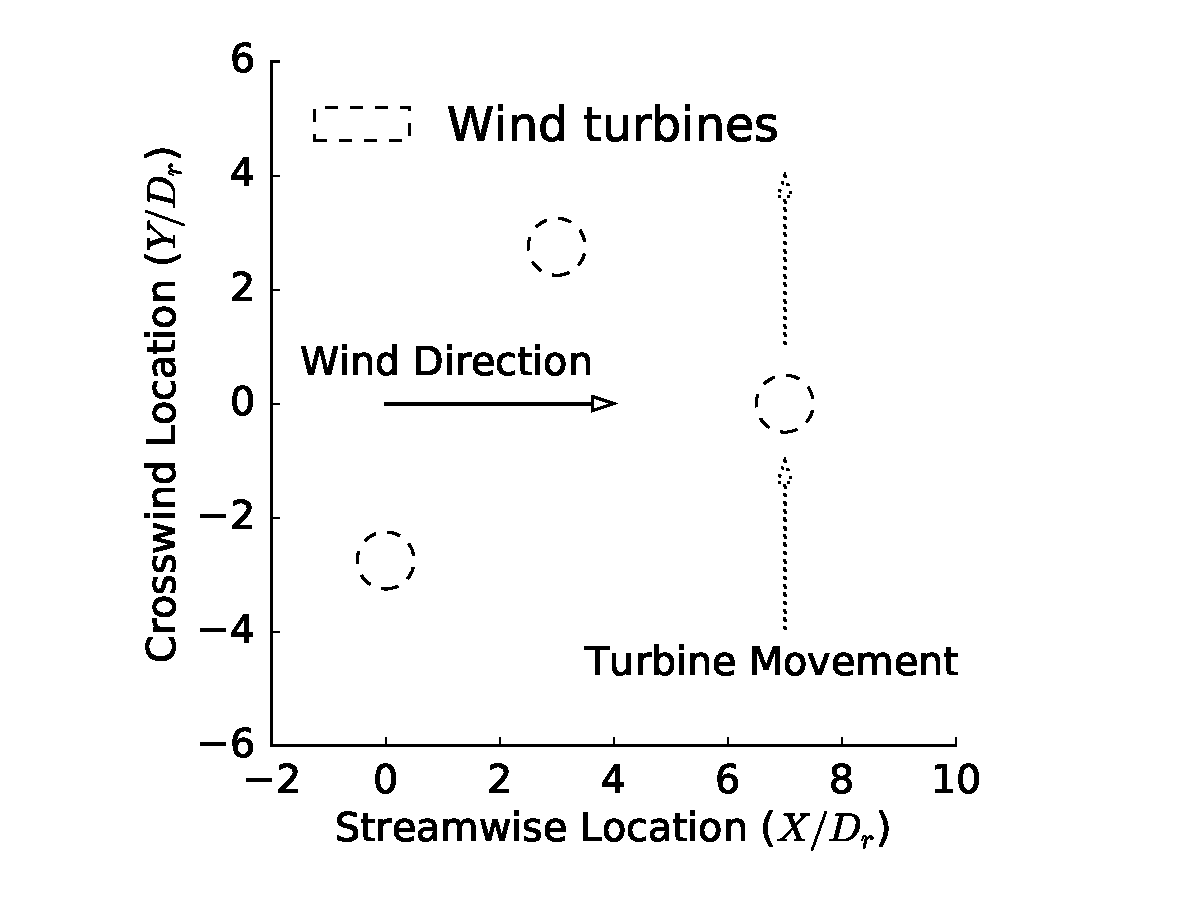
\includegraphics[width=\textwidth, trim={2cm 0cm 2cm 0cm}, clip]{smoothing_locations}
\caption{Simple design space used to demonstrate the effects of the relaxation factor, $\xi$, on the wind farm layout design space (see \cref{fig:smoothing_visualization}).}
\label{fig:smoothing_locations}
\end{minipage}\hspace{1pc}%
\begin{minipage}[t]{0.52\textwidth}
\centering
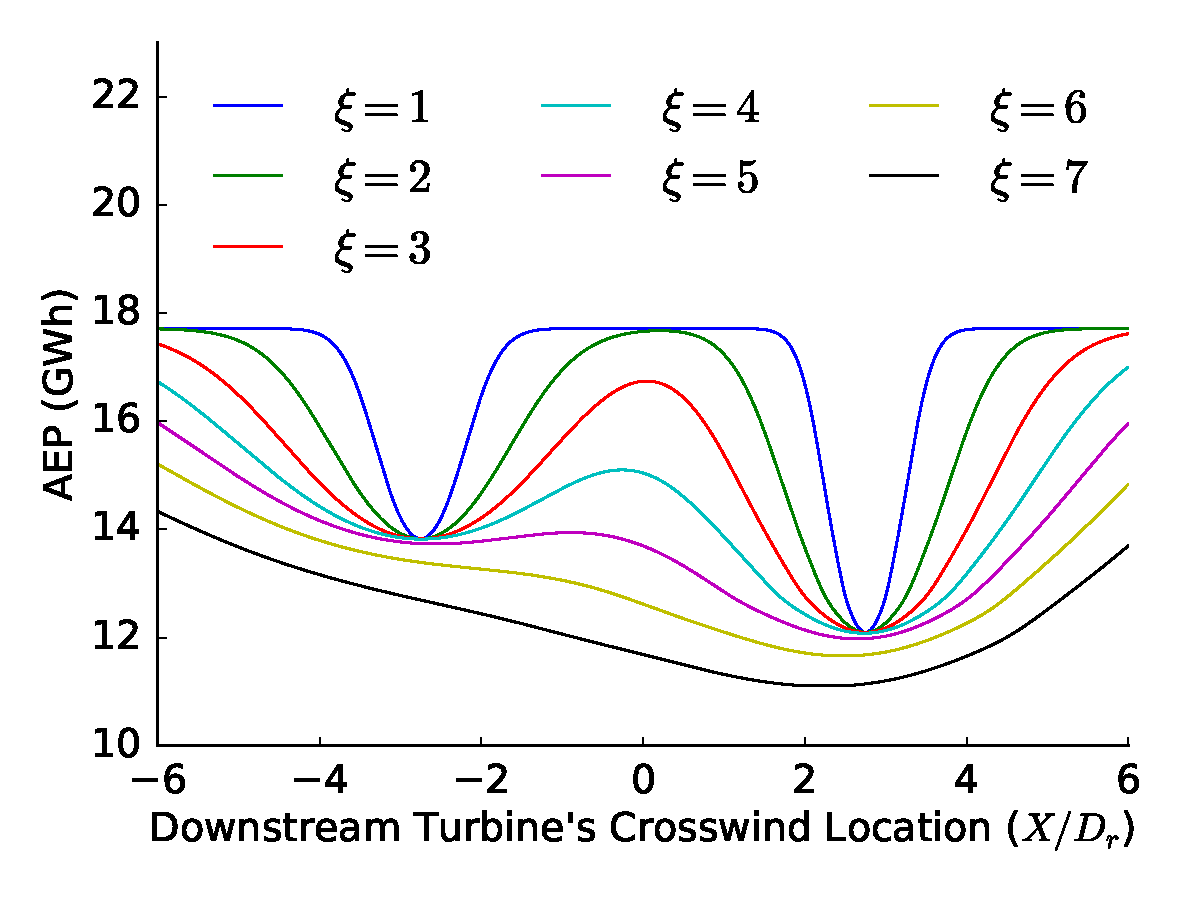
\includegraphics[width=\textwidth]{smoothing_visualization}
\caption{The impact of the relaxation factor, $\xi$, on a simple wind farm layout design space with three turbines and one wind direction. One turbine was moved across the wakes of two upstream turbines (see \cref{fig:smoothing_locations}). }
\label{fig:smoothing_visualization}
\end{minipage} 
\end{figure}
%
\todo{Should the x-axis on \cref{fig:smoothing_visualization} be Y/Dr rather than X/Dr?}

Local optima scattered throughout the design space are reduced as the spaces between wakes are filled with mixed wakes. Larger values of $\xi$ allow the smaller local optima to disappear completely. Smaller values of $\xi$ allow for more accurate wake widths but with an increase in the number and magnitude of local optima. When $\xi$ is set to 1, \cref{eq:bpa_relax} reduces to \cref{eq:bpa}.

\subsection{Bastankhah and Port\'e-Agel WEC Step (3)}
To gain the benefits of WEC without losing the accuracy of the wake model, the optimization must be run multiple times, in a continuation approach, with values of $\xi$ decreasing to unity. The results from optimizing with each value of $\xi$ can then be used to warm start the next optimization. In this way, the gradient-based optimization can intelligently explore the design space and then refine the model to find a final, more accurate, result. The interative optimizations are generally fairly fast due to starting from the previous optimized solution, so WEC does not necessarily take as long to run as an equal number of independent optimizations. For the optimization results presented in this paper, $\xi$ took on the values [3, 2.75, 2.5, 2.25, 2.0, 1.75, 1.5, 1.25, 1.0]. These values were selected primarily through trial and error. The selection of these values should be investigated in more depth in future work.
\todo{is there a typo here? "The \textbf{interative} optimizations are generally..."}

\section{Test Cases and Optimization}
To demonstrate the effectiveness of WEC, we present two wind farm optimization cases. For both cases, we used the Vestas V-80 2MW wind turbine. The cases were chosen to represent a range in the size, complexity, and difficulty of the optimization problem.

We created 199 pseudo-random starting wind farm layouts for each case. Each of the starting layouts had all the turbines inside the wind farm boundary constraint and did not have any turbine spacings less than one rotor diameter. These starting locations, along with the planned locations shown in \cref{fig:grid_case,fig:round_case}, served as the 200 starting locations for the optimizations.

To set up the optimizations, we used OpenMDAO: a computing platform for systems analysis and multidisciplinary optimization \cite{gray2010_OpenMDAO}. The optimizations were solved using SNOPT, a sparse non-linear optimization algorithm \cite{gill2005}; WEC with SNOPT as the optimization algorithm; 
%ALPSO, an augmented Lagrangian particle swarm optimization approach \cite{jansen2011_alpso}; %
and NSGA-II, a non-dominated sorting genetic algorithm \cite{deb2002_nsga2}. Both of the optimization algorithms were used as implemented in PyOptSparse \cite{ruben2012_pyopt}, except that a simple tolerance for convergence was added to NSGA-II. The added tolerance in NSGA-II required that the best solution not change more than some specified value for a minimum number of generations. 

For each test case, the population size for NSGA-II was set to be ten times the number of design variables ($10\times N_{turbines} \times 2$) and the convergence tolerance was set to be $1\times10^{-4}$. The simulation was considered converged if the objective function value did not change more than the convergence tolerance for 100 or 200 consecutive generations for case 1 and case 2 respectively. Total generations were mostly in the thousands for each optimization run.

\subsection{Case 0: Single Dimension}
\todo{Spencer}
The case 0 tests were designed to place either one or two permanent turbines upwind of a variable downwind turbine. This downwind turbine was traversed in the crosswind direction through the wakes of each upwind turbine. The AEP was recorded as the downwind turbine was traversed through the wakes of the upwind turbines. This process was repeated for multiple relaxation factors, and the resulting AEP curves were plotted.

%The preliminary goals of this study were to determine whether WEC (1) spread out the wake for each wake model and (2) maintained the velocity deficit at the wake's center for each wake model. The case 0 tests were designed to place either one or two permanent turbines upwind of a variable downwind turbine. This downwind turbine was traversed in the crosswind direction through the wakes of each upwind turbine. The AEP was recorded as the downwind turbine was traversed through the wakes of the upwind turbines. This process was repeated for multiple relaxation factors, and the resulting AEP curves were plotted.

\subsection{Case 0.5: Small-Scale Optimization}
\todo{Jared: what do you think of this section? It's for the small-scale optimization tests we ran}
Once the preliminary tests had been completed, case 0.5 was ran to predict whether the intended effects of WEC---that turbines would be optimized to better optima rather than local optima between wakes---would be realized in our large-scale optimizations. Similar to case 0, two turbines were given constant coordinates upwind of a variable downwind turbine. The coordinates of the variable downwind turbine were optimized to maximize AEP.

\subsection{Case 1: Small Grid}
Case 1 was carefully selected to provide a meaningful problem that would be tractable for all the optimization methods. We defined a wind farm with 16 wind turbines and a square boundary with enough space for four rows and columns of wind turbines with spacings of five rotor diameters (see \cref{fig:grid_case}). We used a simple wind rose composed of a double Gaussian distribution binned into 20 directions and a constant wind speed of 10 m/s in all directions (see \cref{fig:directional}).
\begin{figure}[h!]
\centering
\begin{minipage}[t]{18pc}
\centering
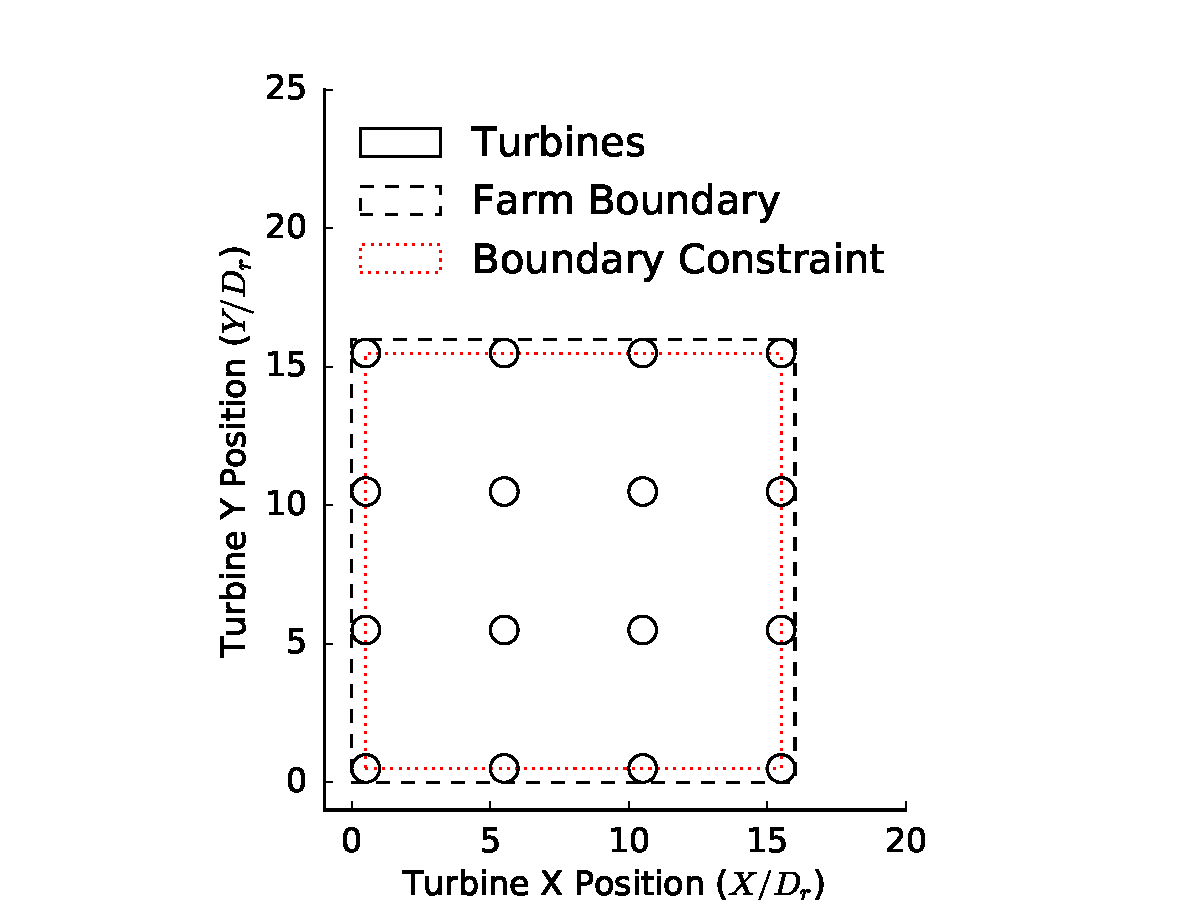
\includegraphics[width=1.\textwidth, trim={3cm, 0cm, 3cm, 0cm}, clip]{final_images/grid_farm_16Turbines_5DSpacing_start.pdf}
\caption{Baseline wind farm layout for case 1. The circles marking turbine locations are to scale, with diameters equal to the rotor diameter.}
\label{fig:grid_case}
\end{minipage}\hspace{1pc}%
\begin{minipage}[t]{18pc}
\centering
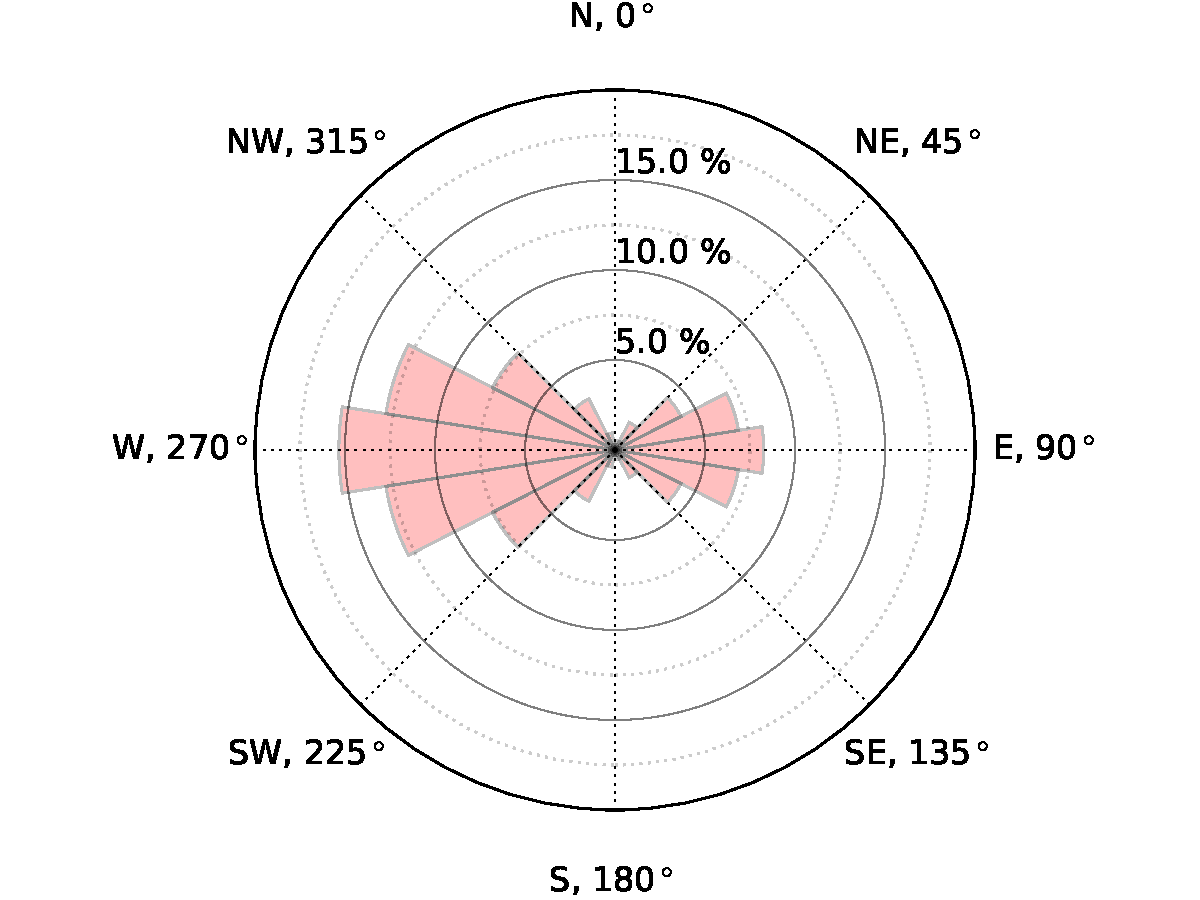
\includegraphics[width=\textwidth, trim={1.5cm 0cm 1.5cm 0cm}, clip]{final_images/directional_windrose.pdf}
\caption{Direction probability wind rose for case 1. This wind rose is composed of a double Gaussian distribution binned into 20 directions.}
\label{fig:directional}
\end{minipage} 
\end{figure}
%

For case 1, the optimization problem was formulated as shown in \cref{eqn:opt1}
%
\begin{equation}
	\label{eqn:opt1}
	\begin{aligned} [b]
	\underset{x_i,y_i}{\textrm{maximize}} \quad & AEP(x_i,y_i,)~~i=1...16\\
	\textrm{subject to} \quad & S_{i,j} \geq 2\*D_{r}~~i,j=1...16,~~i \neq j\\
	 & x_{min} \leq x_i \leq x_{max}~~i=1...16\\
     & y_{min} \leq y_i \leq y_{max}~~i=1...16\\
	\end{aligned}
\end{equation}
%
Where $(x_i,y_i)$ is the position of each turbine $i$, $S_{i,j}$ represents the separation distance between each pair of turbines $i$ and $j$, and $x_{max/min}$ and $y_{max/min}$ represent the boundaries of the wind farm. This case has a total of 32 variables and 120 constraints.

\subsection{Case 2: Round Farm}
\begin{figure}[h!]
\centering
\begin{minipage}[t]{18pc}
\centering
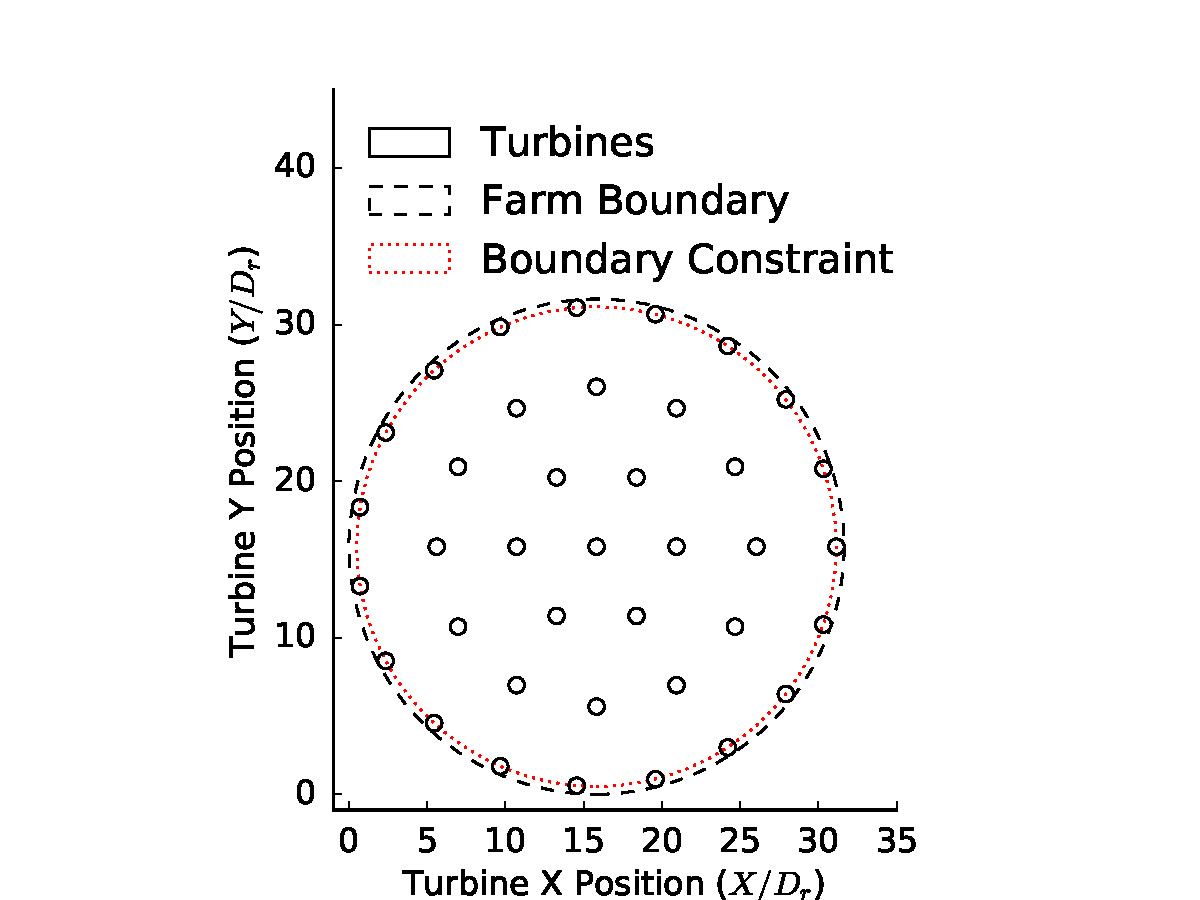
\includegraphics[width=\textwidth, trim={3cm, 0cm, 3cm, 0cm}, clip]{final_images/round_farm_38Turbines_5DSpacing_start.pdf}
\caption{Baseline wind farm layout for case 2. The circles marking turbine locations are to scale, with diameters equal to the rotor diameter.}
\label{fig:round_case}
\end{minipage}\hspace{1pc}%
\begin{minipage}[t]{18pc}
\centering
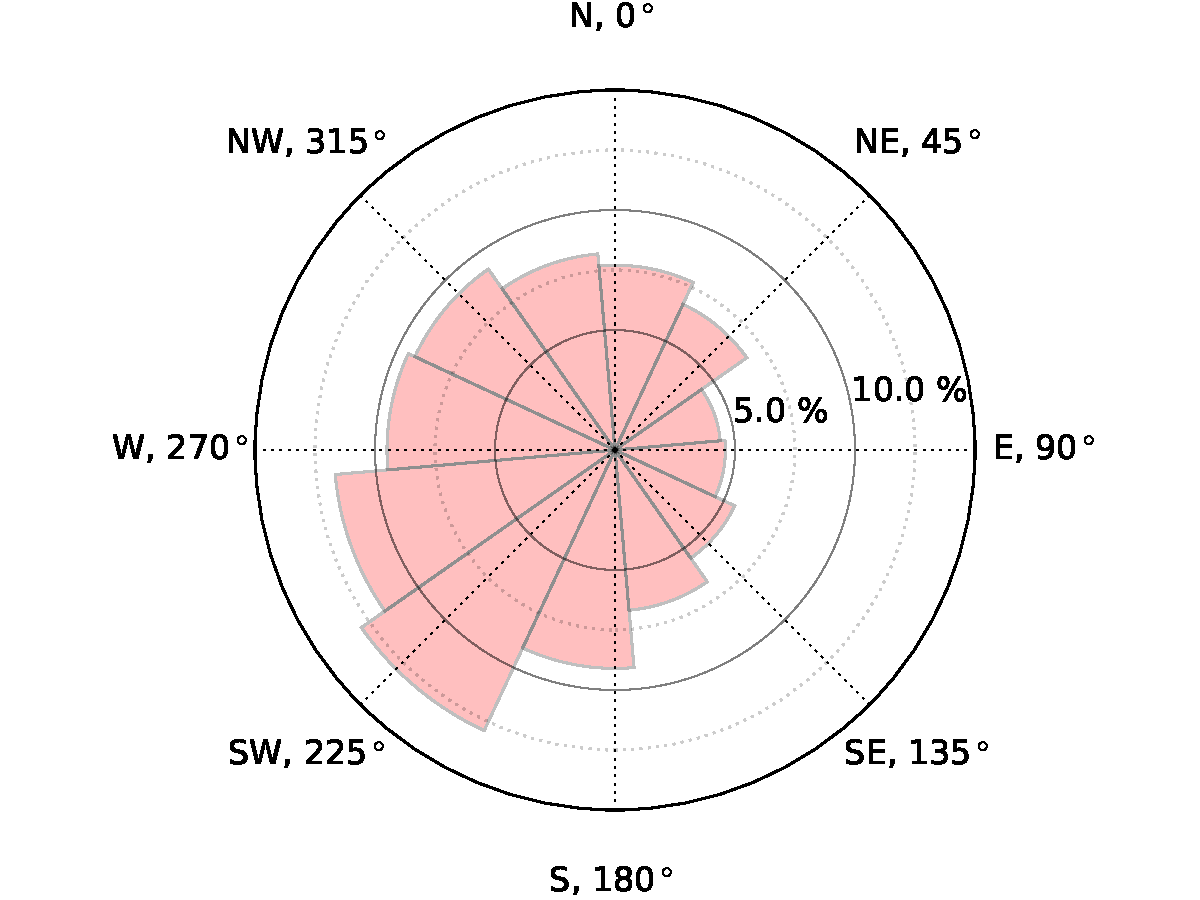
\includegraphics[width=\textwidth, trim={1.5cm 0cm 1.5cm 0cm}, clip]{final_images/nantucket_windrose.pdf}
\caption{Directional probability wind rose for case 2. This is the Nantucket wind rose binned into 12 directions \cite{wrcc2017}.}
\label{fig:nantucket}
\end{minipage} 
\end{figure}

  Case 2 was created to be significantly more challenging than the first case. We defined a wind farm with 38 wind turbines and a circular boundary (see \cref{fig:round_case}). The size of the boundary allowed for at least a five-diameter spacing between turbines. We used a simplified version of the Nantucket wind rose binned into 12 directions with a constant wind speed of 10 m/s in all directions (see \cref{fig:nantucket}).


The optimization problem for case 2 was formulated as
%
\begin{equation}
	\label{e:objective}
	\begin{aligned} [b]
	\underset{x_i,y_i}{\textrm{maximize}} \quad & AEP(x_i,y_i,)~~i=1...38\\
	\textrm{subject to} \quad & S_{i,j} \geq 2\*D_{r}~~i,j=1...38~~i \neq j\\
	 & [x_c-x_i]^2+[y_c-y_i]^2 \leq R_{b}^2~~i=1...38\\
	\end{aligned}
\end{equation}
%
where $(x_c,y_c)$ is the location of the center of the wind farm, and $R_b$ is the radius of the wind farm boundary. This case has a total of 76 variables and 741 constraints.

\section{Results}\label{sec:results}
\todo{Jared: figure out how to best present these results now that we have 3 models}
We compared optimized AEP, as well as the number of function calls required, for each of the cases discussed previously. We used function calls as a surrogate for time. We did not report wall time because we did not maintain enough consistency in the computational resources used for each optimization run (cores, processor types, computational isolation, etc). Results for each test case will be presented and discussed in the following sections.

%\subsection{Case 0 Results}
%Results for case 0 can be seen in \cref{fig:WECAEPFigures}. As the relaxation factor increases in the left-hand plots, the wake's effects are felt farther from the wake center (i.e., the wake expands). An important feature displayed by the right-hand column is that the local maxima are being smoothed out. This key result allows gradient-based optimizations to avoid converging on most local maxima.

%\todo{Spencer: may need to update some of these figures}
% Enter subfigures of AEP vs. crosswind position displaying widening effects of WEC.
% \begin{figure}[htbp!]
%\begin{figure}[H]
%    \centering
%    \subfigure[]{
%        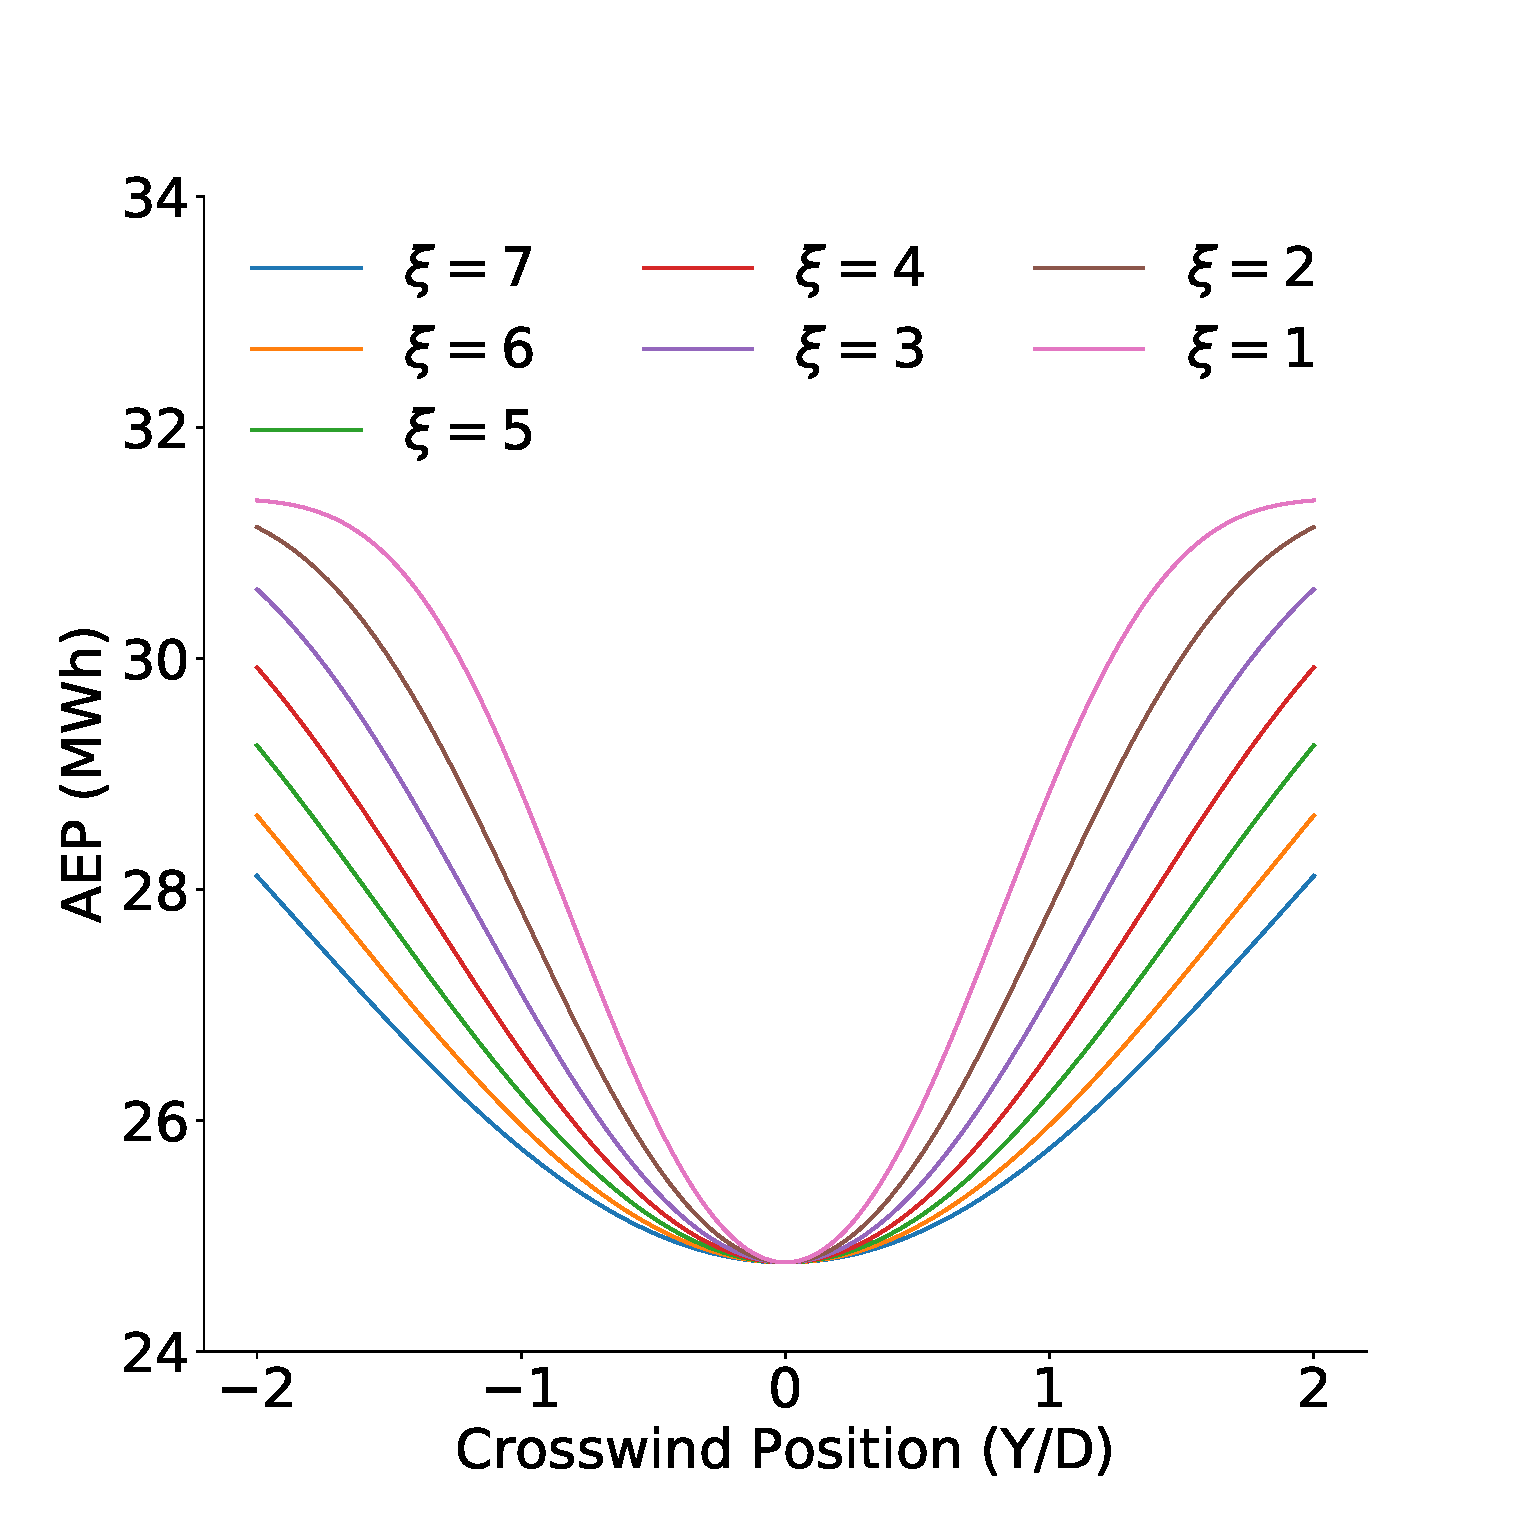
\includegraphics[width=0.4\textwidth, trim={0cm 1cm 0cm 1cm}]{JensenWECSingleTurbineAEP.eps}
%    }
%    \subfigure[]{
%        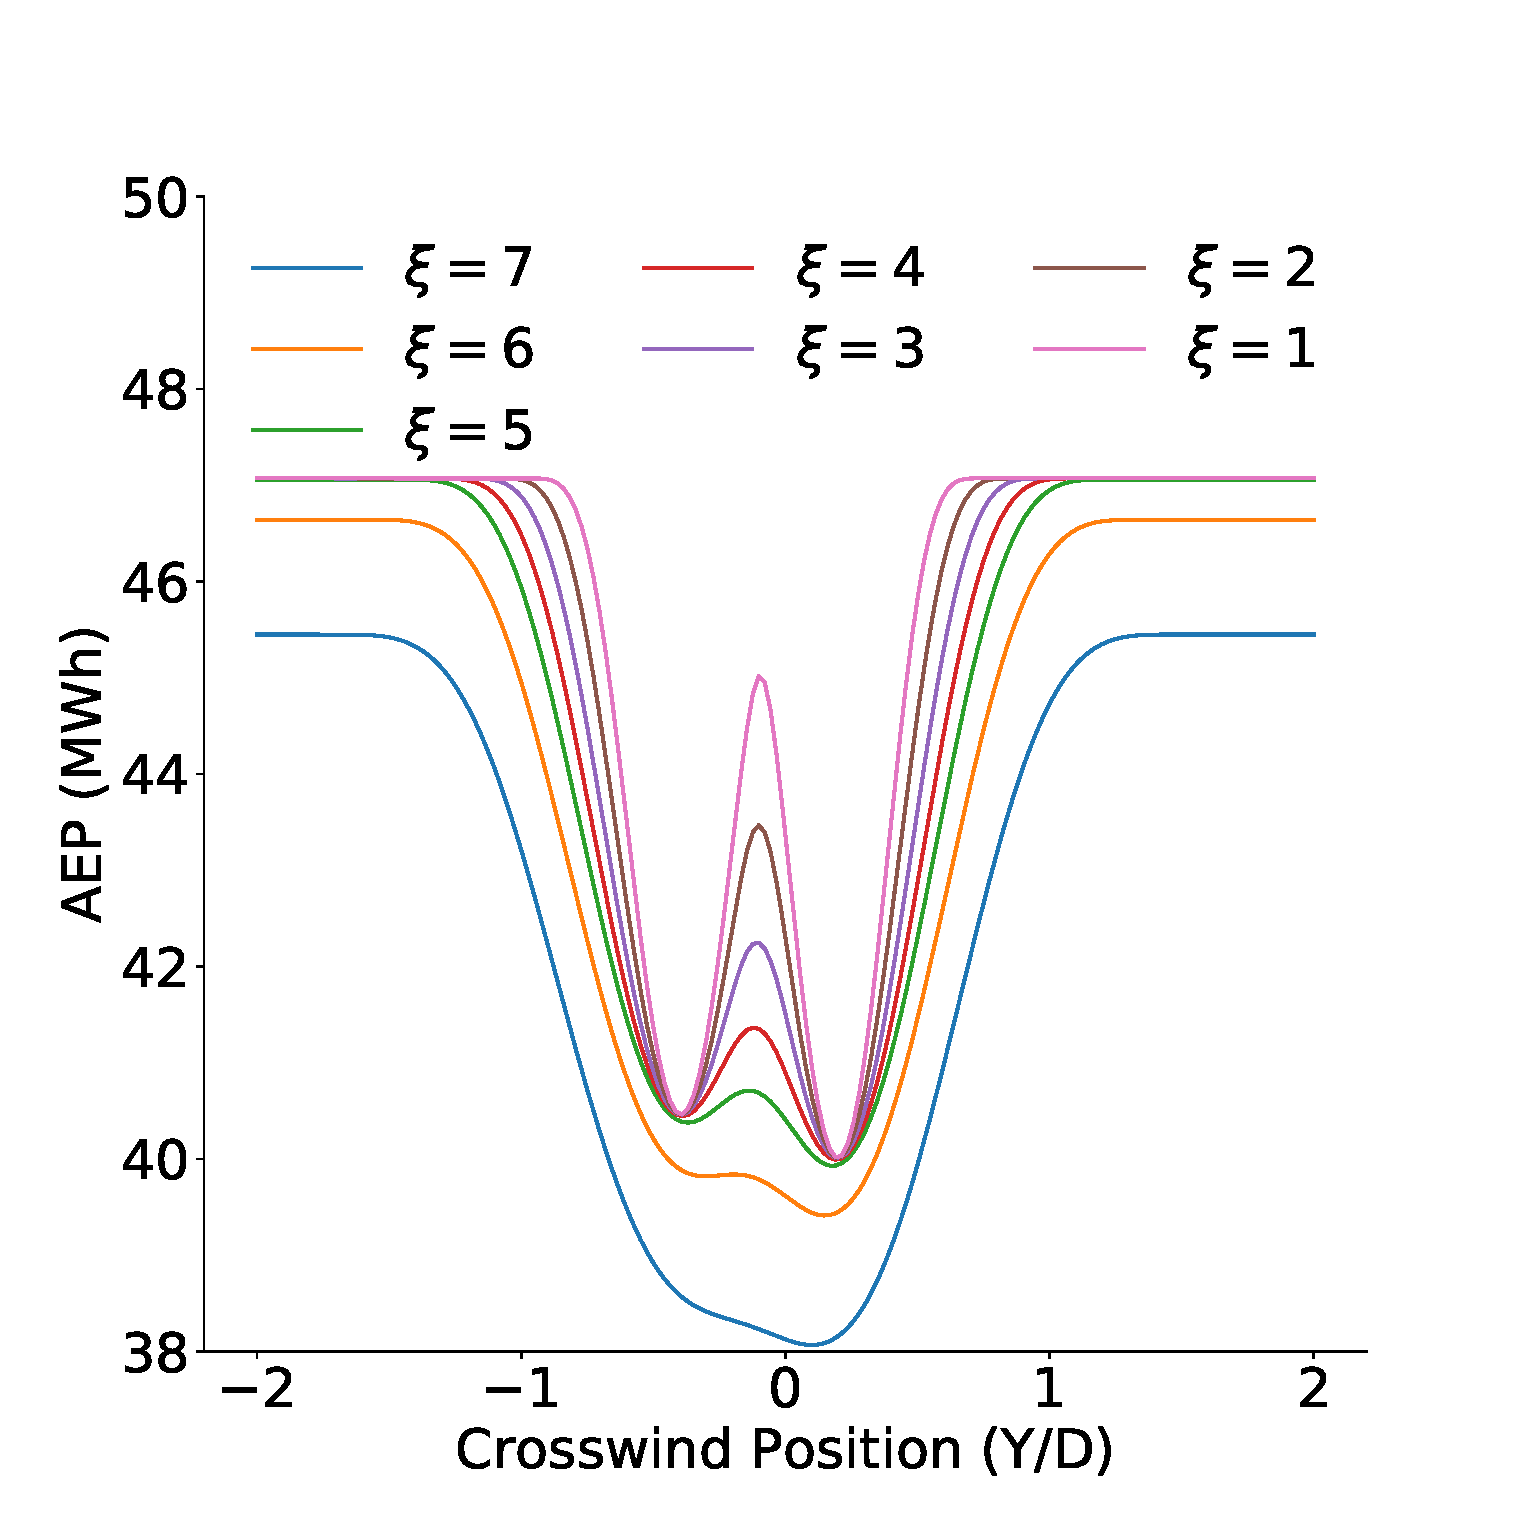
\includegraphics[width=0.4\textwidth, trim={0cm 1cm 0cm 1cm}]{JensenWECMultipleTurbinesAEP.eps}
%    }
%    \subfigure[]{
%        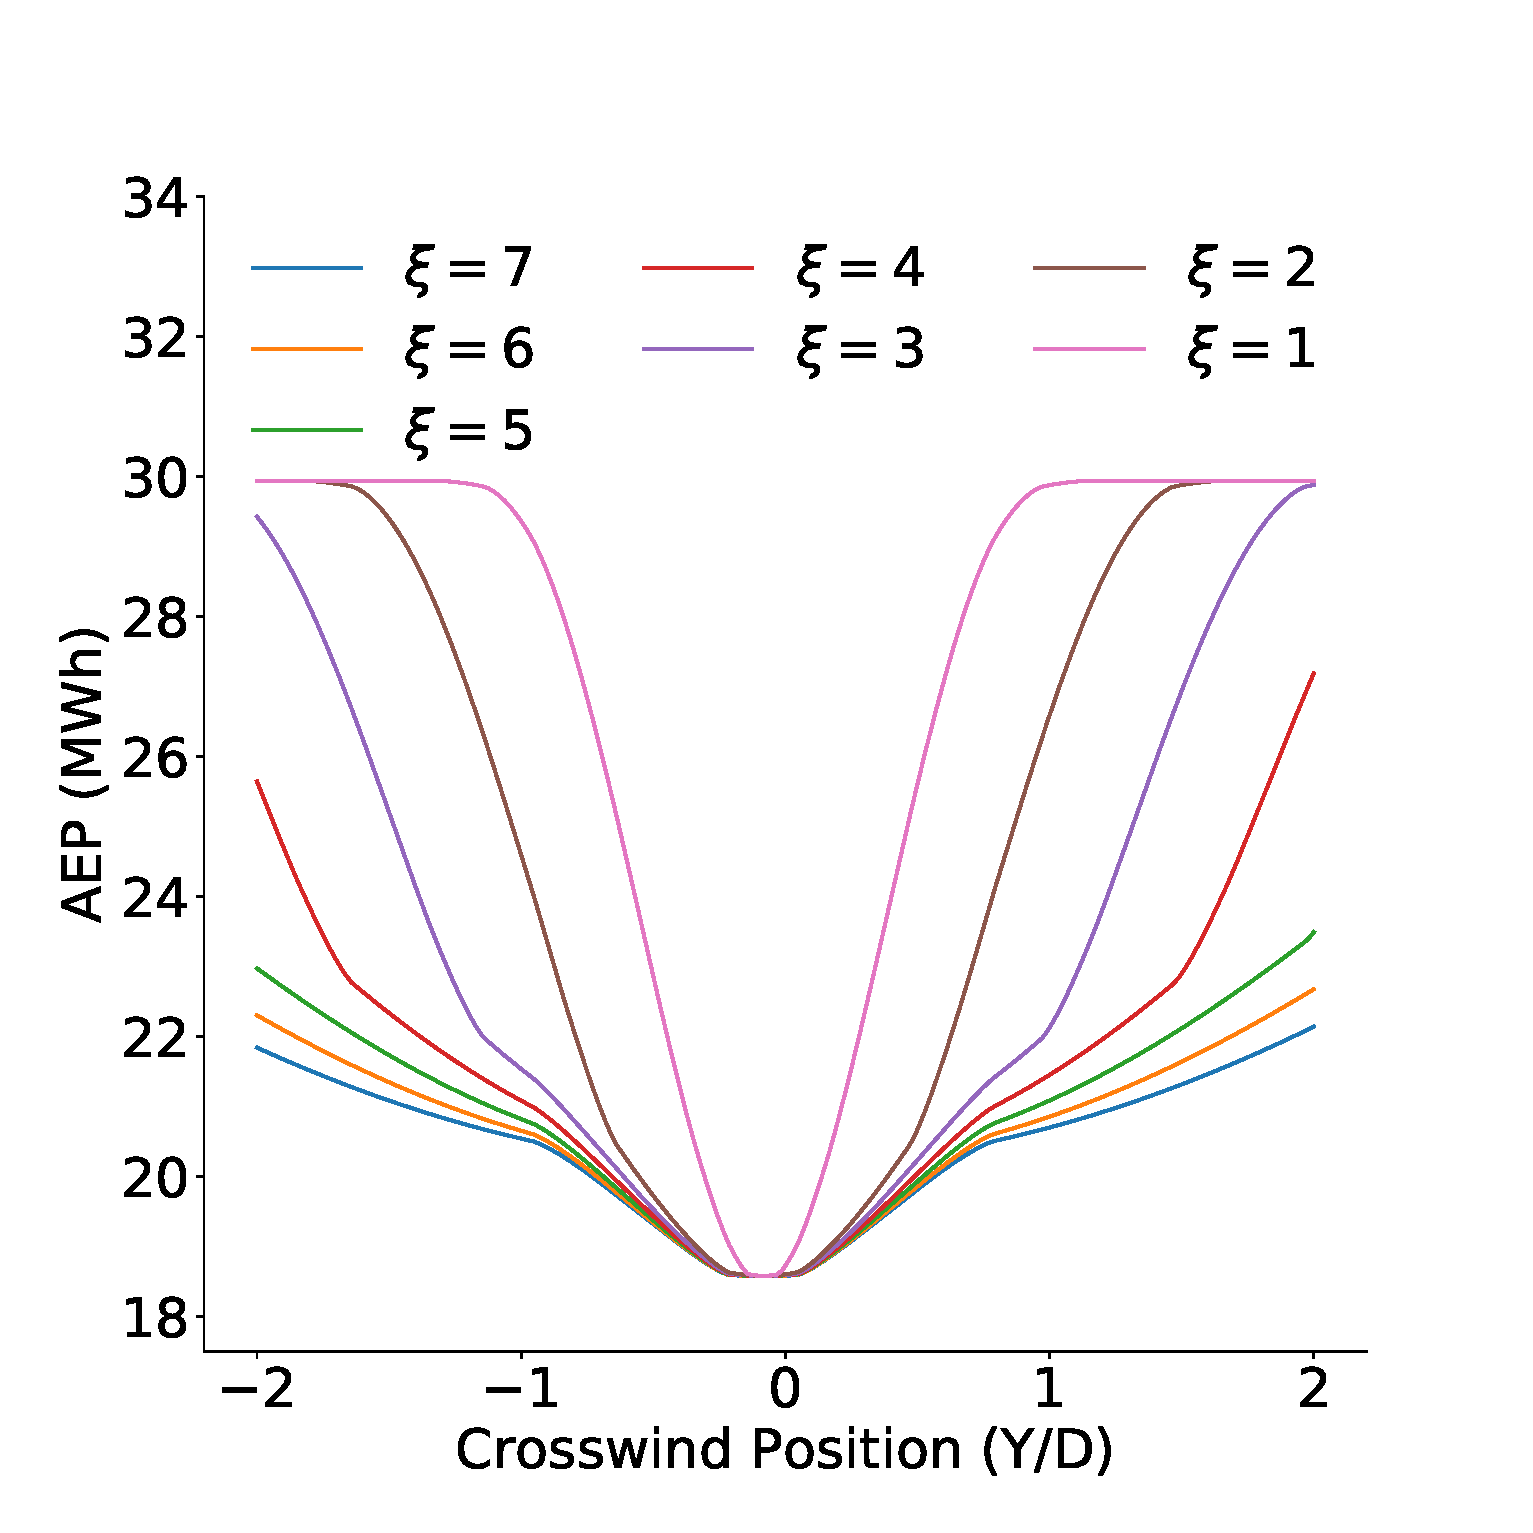
\includegraphics[width=0.4\textwidth, trim={0cm 1cm 0cm 1cm}]{FLORISWECSingleTurbineAEP.eps}
%    }
%    \subfigure[]{
%        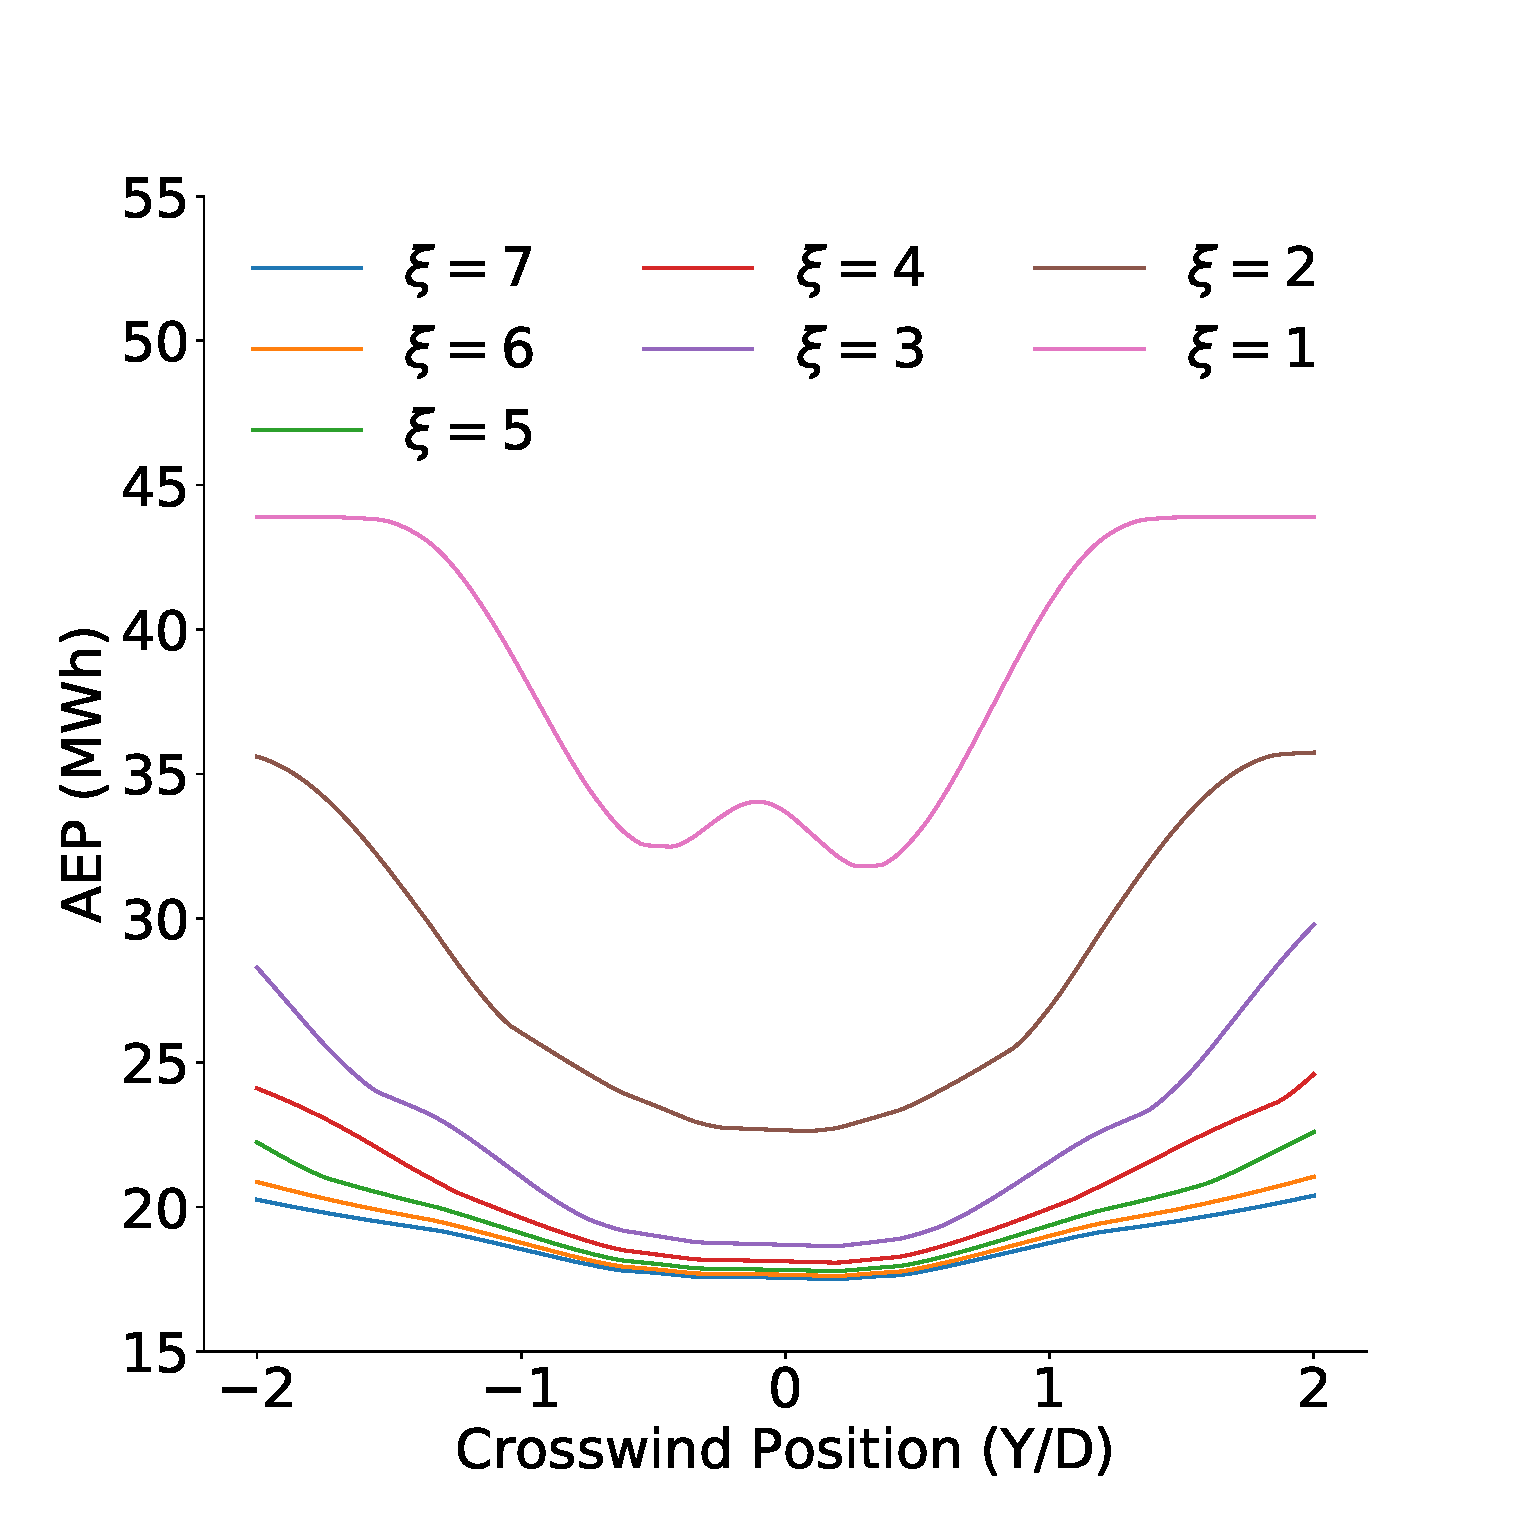
\includegraphics[width=0.4\textwidth, trim={0cm 1cm 0cm 1cm}]{FLORISWECMultipleTurbinesAEP.eps}
%    }
%    \subfigure[]{
%        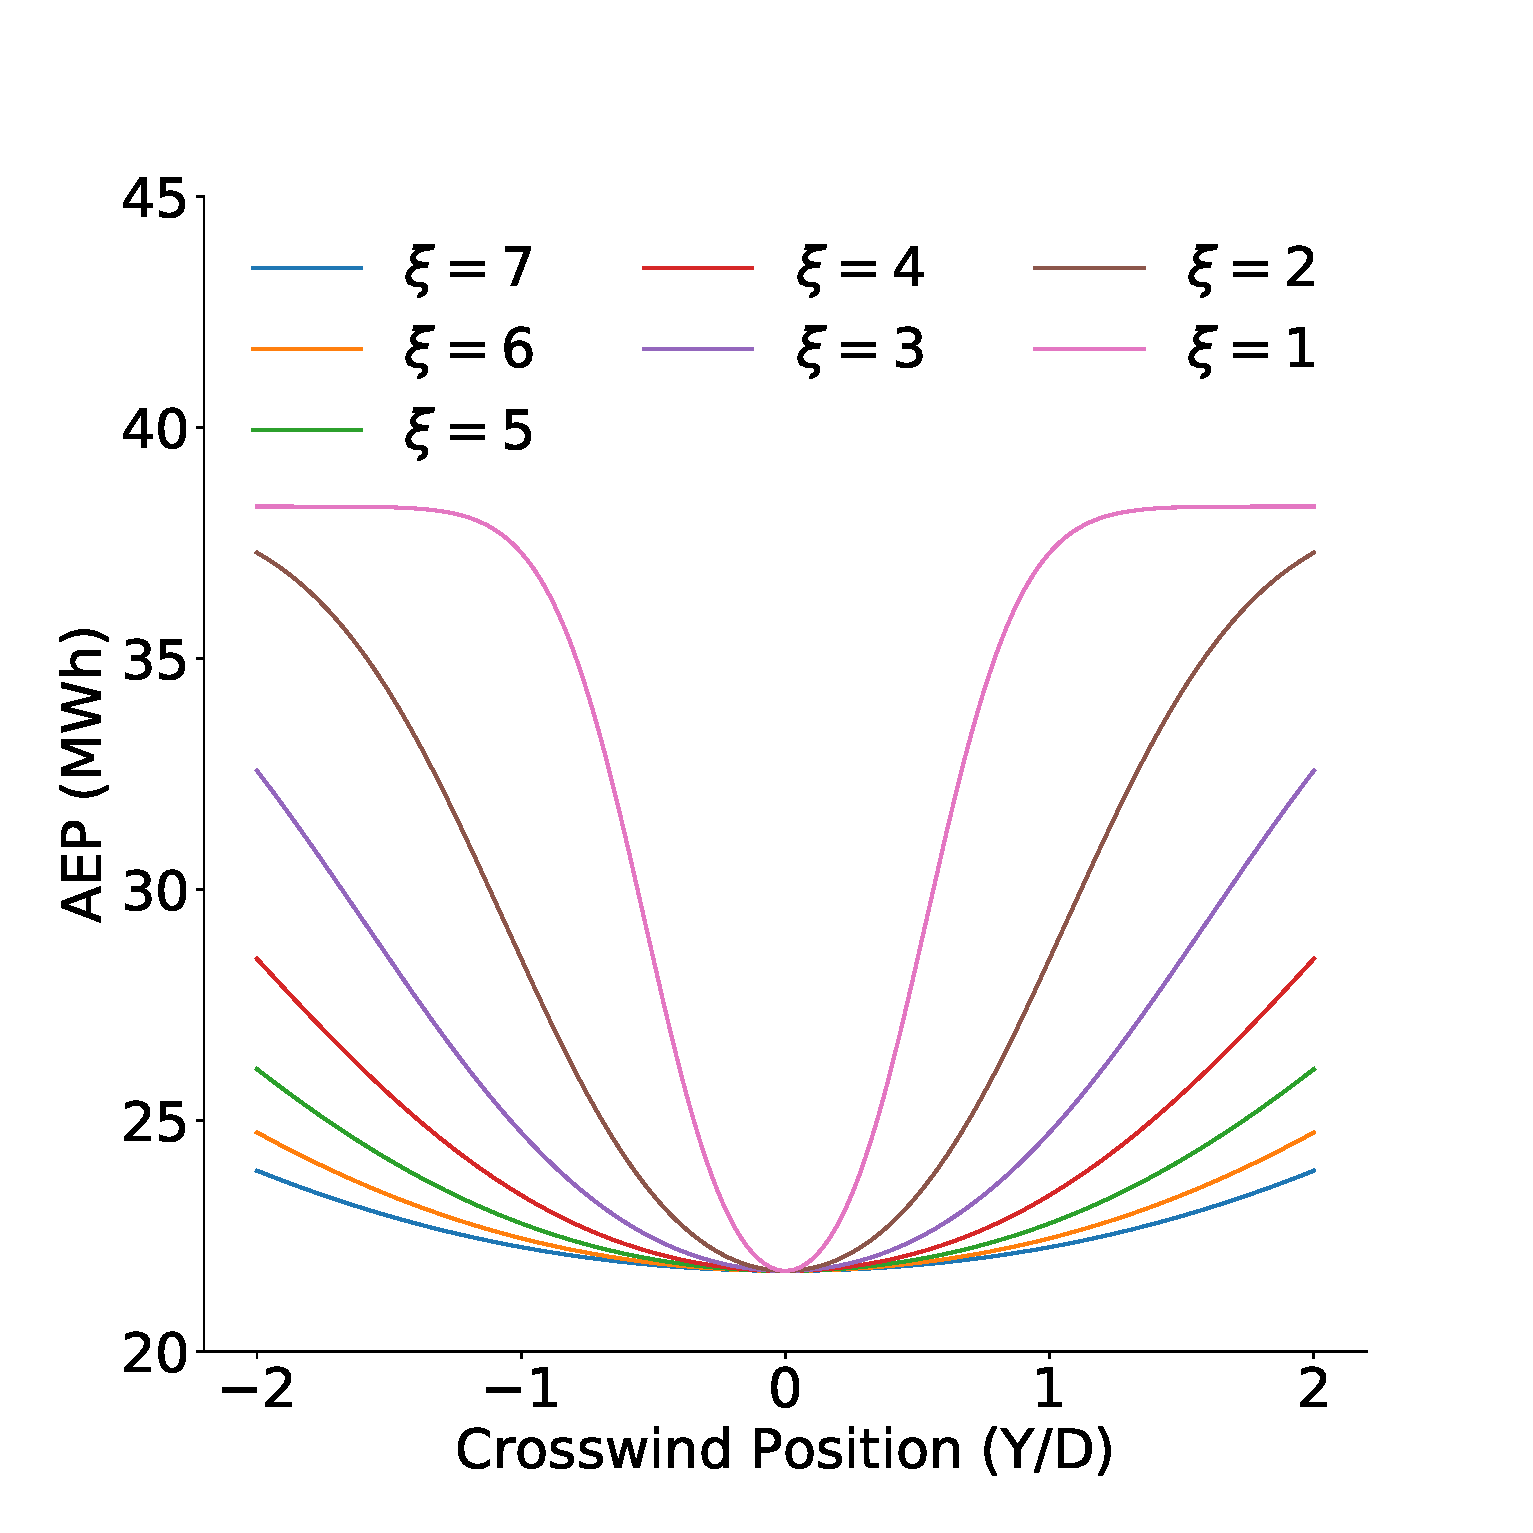
\includegraphics[width=0.4\textwidth, trim={0cm 1cm 0cm 1cm}]{BastankhahWECSingleTurbineAEP.eps}
%    }
%    \subfigure[]{
%        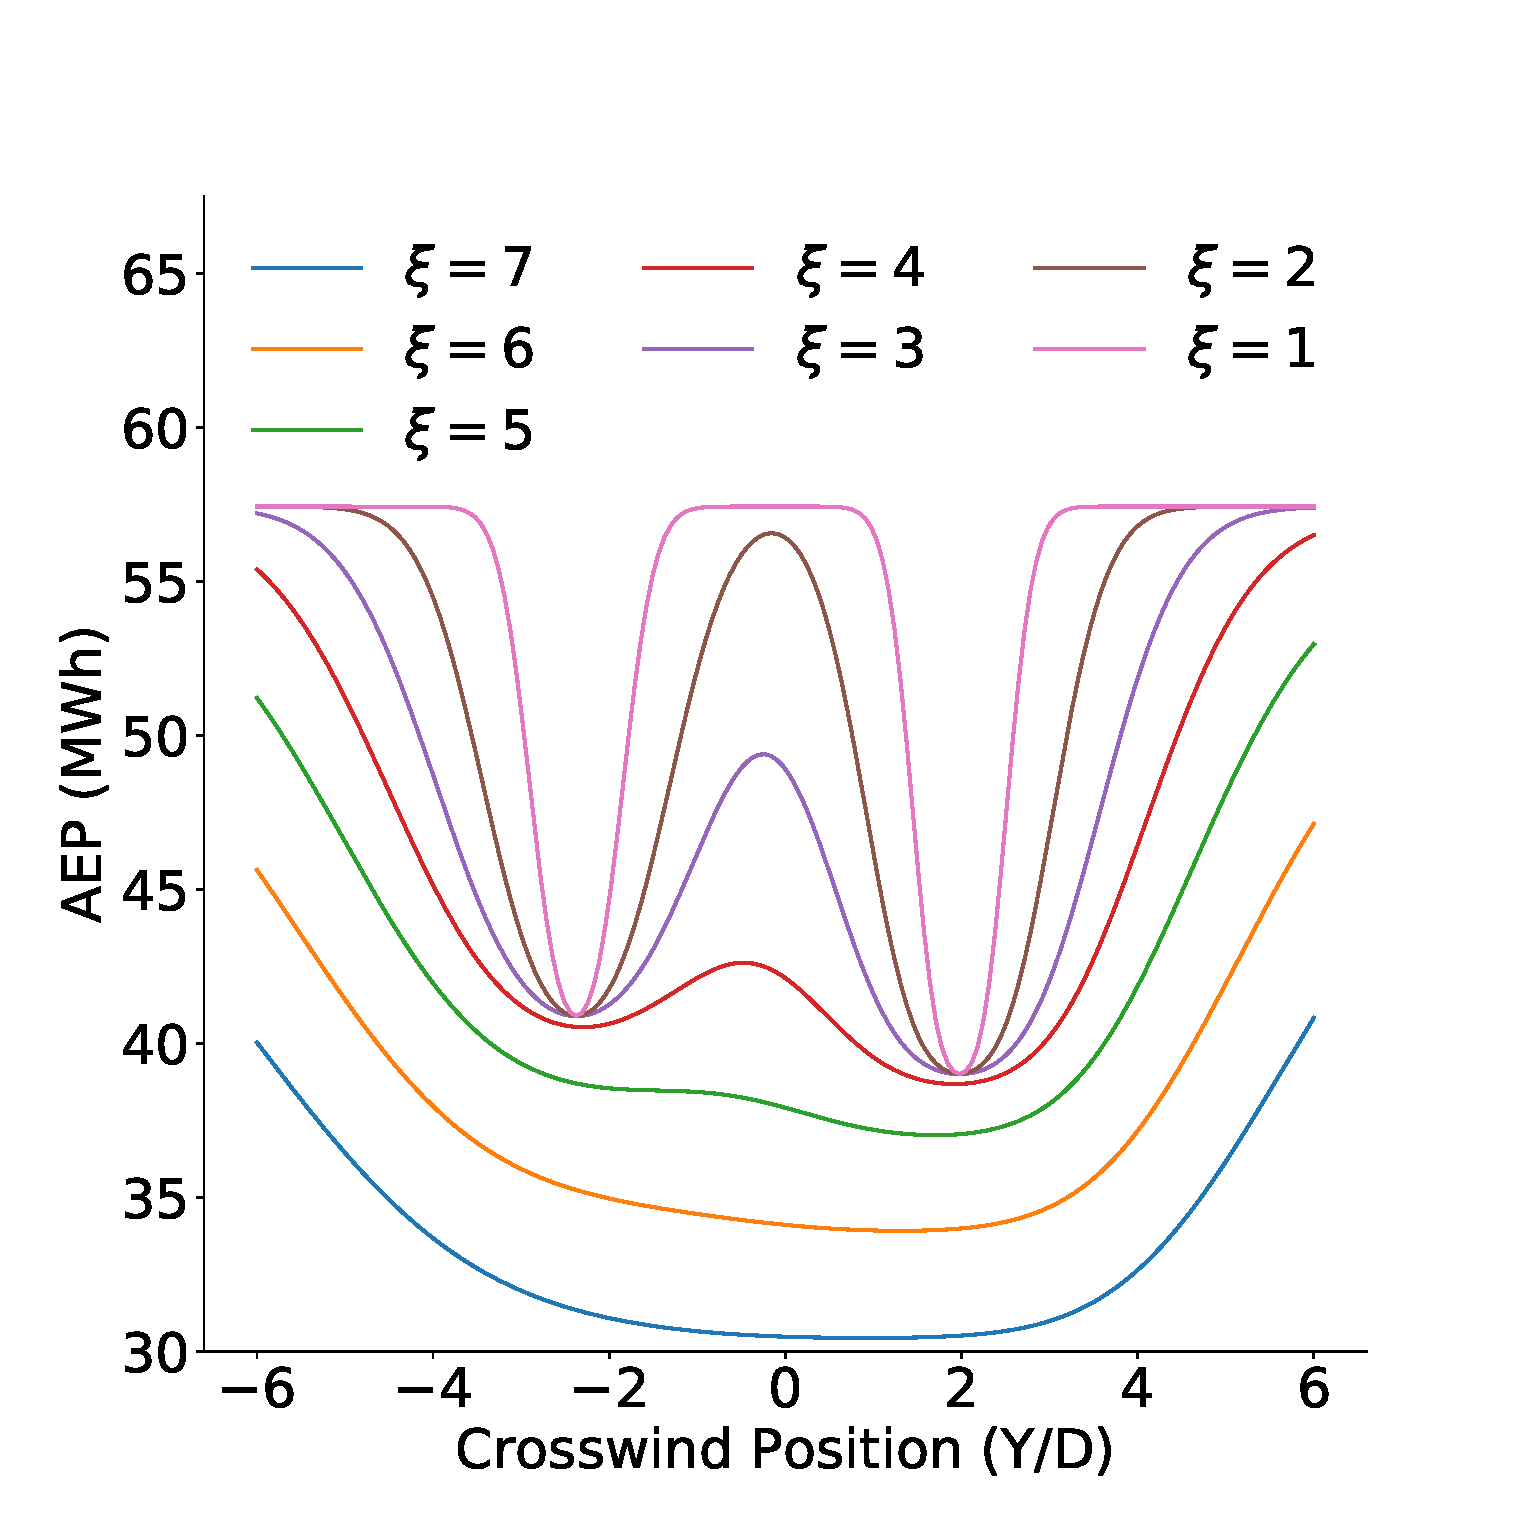
\includegraphics[width=0.4\textwidth, trim={0cm 1cm 0cm 1cm}]{BastankhahWECMultipleTurbinesAEP.eps}
%    }
%    \caption{Plots displaying the effects the WEC approach has on wake width. Plots (a) and (b) display the Jensen-Cosine model, plots (c) and (d) display the FLORIS model, and (e) and (f) display the BPA model.}
%    \label{fig:WECAEPFigures}
%\end{figure}

\subsection{Case 0 Results}
\todo{Spencer: finish this section}

Results for case 0 are displayed below. Note that optimizations without WEC fail to escape the local optimum between wakes, whereas optimizations with WEC place the downwind turbine in a more optimal location for each wake model.

\todo{refer to notes from Jared in updating these figures.}
\begin{figure}[H]
    \centering
    \subfigure[]{
        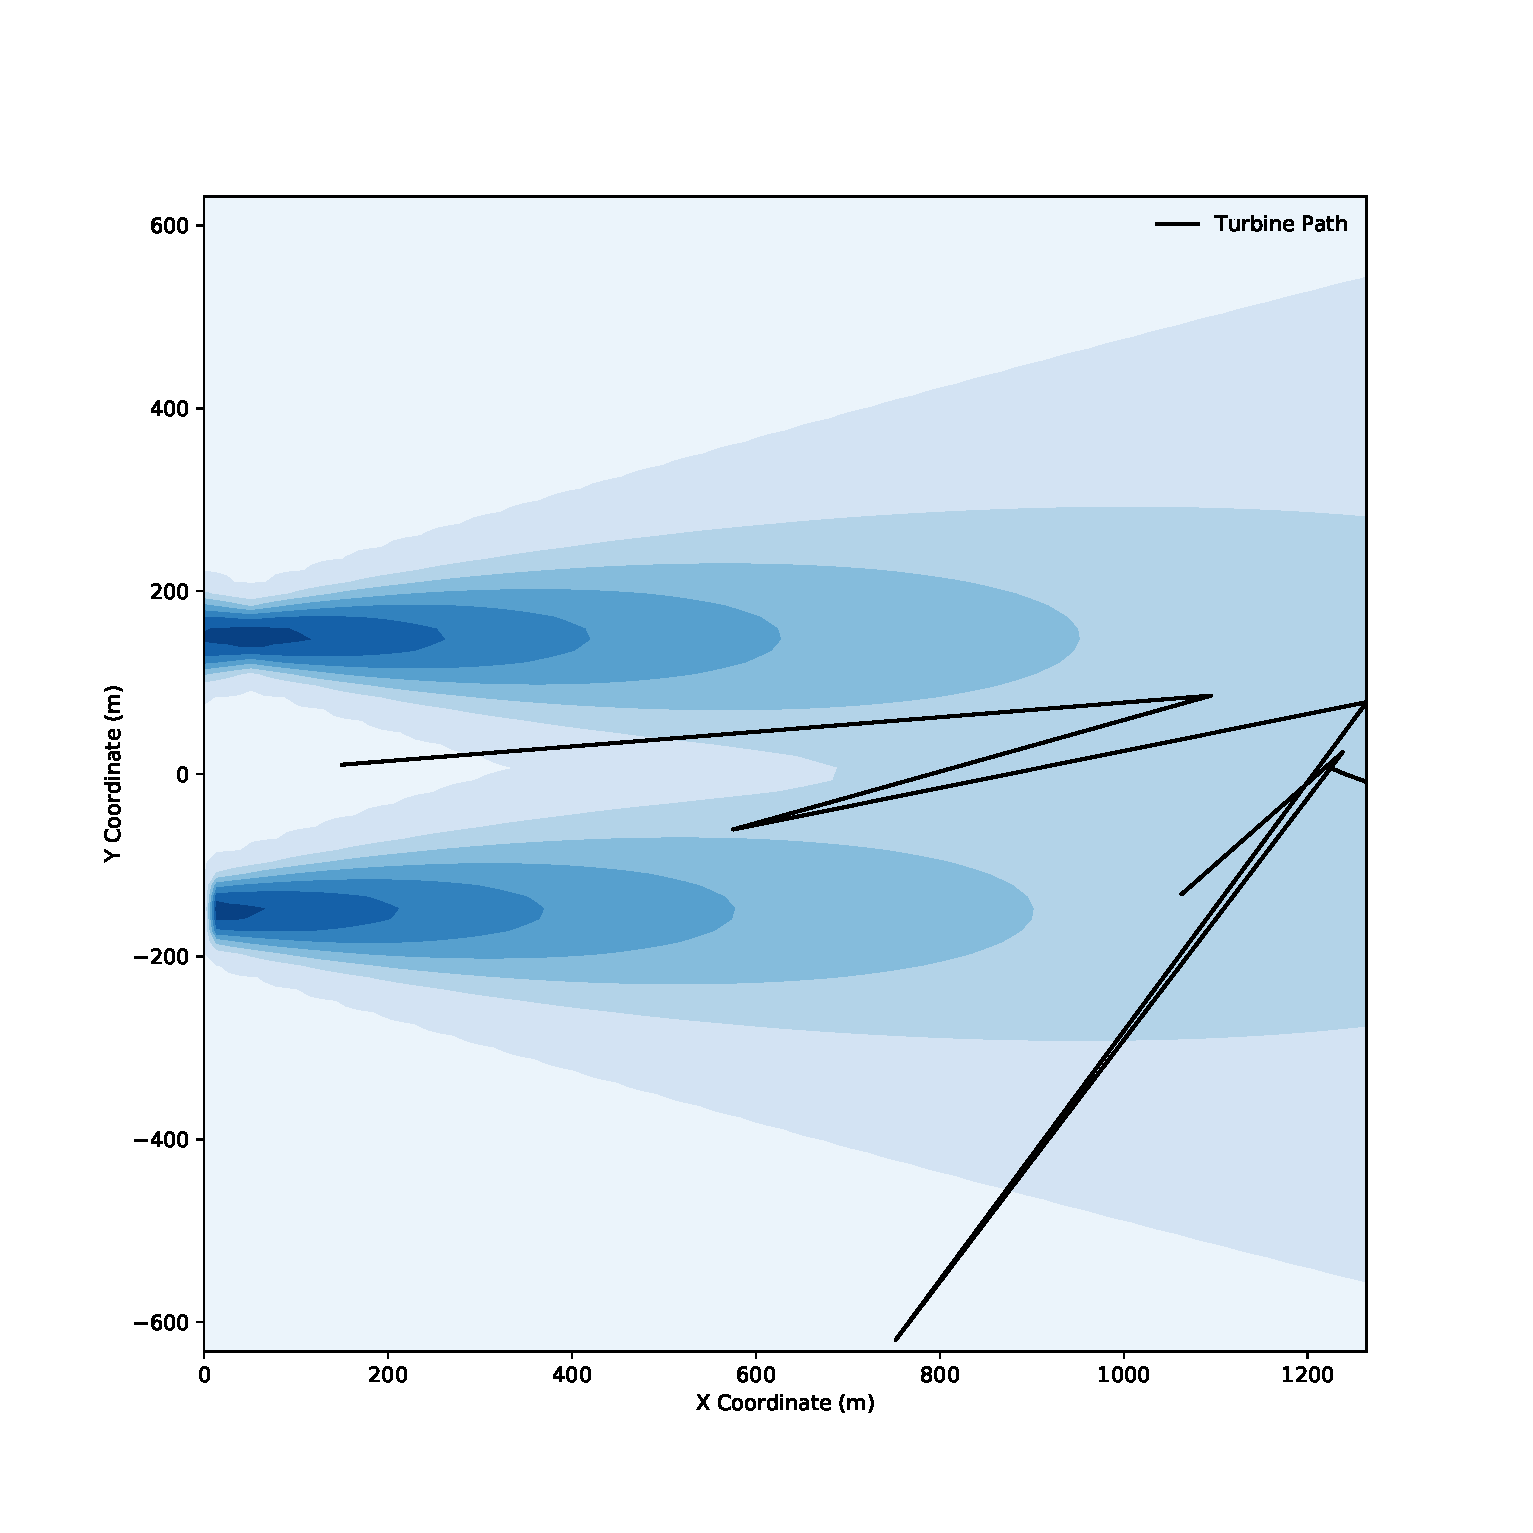
\includegraphics[width=0.35\textwidth]{SmallScaleJensenNonWECGraphContour}
    }
    \subfigure[]{
        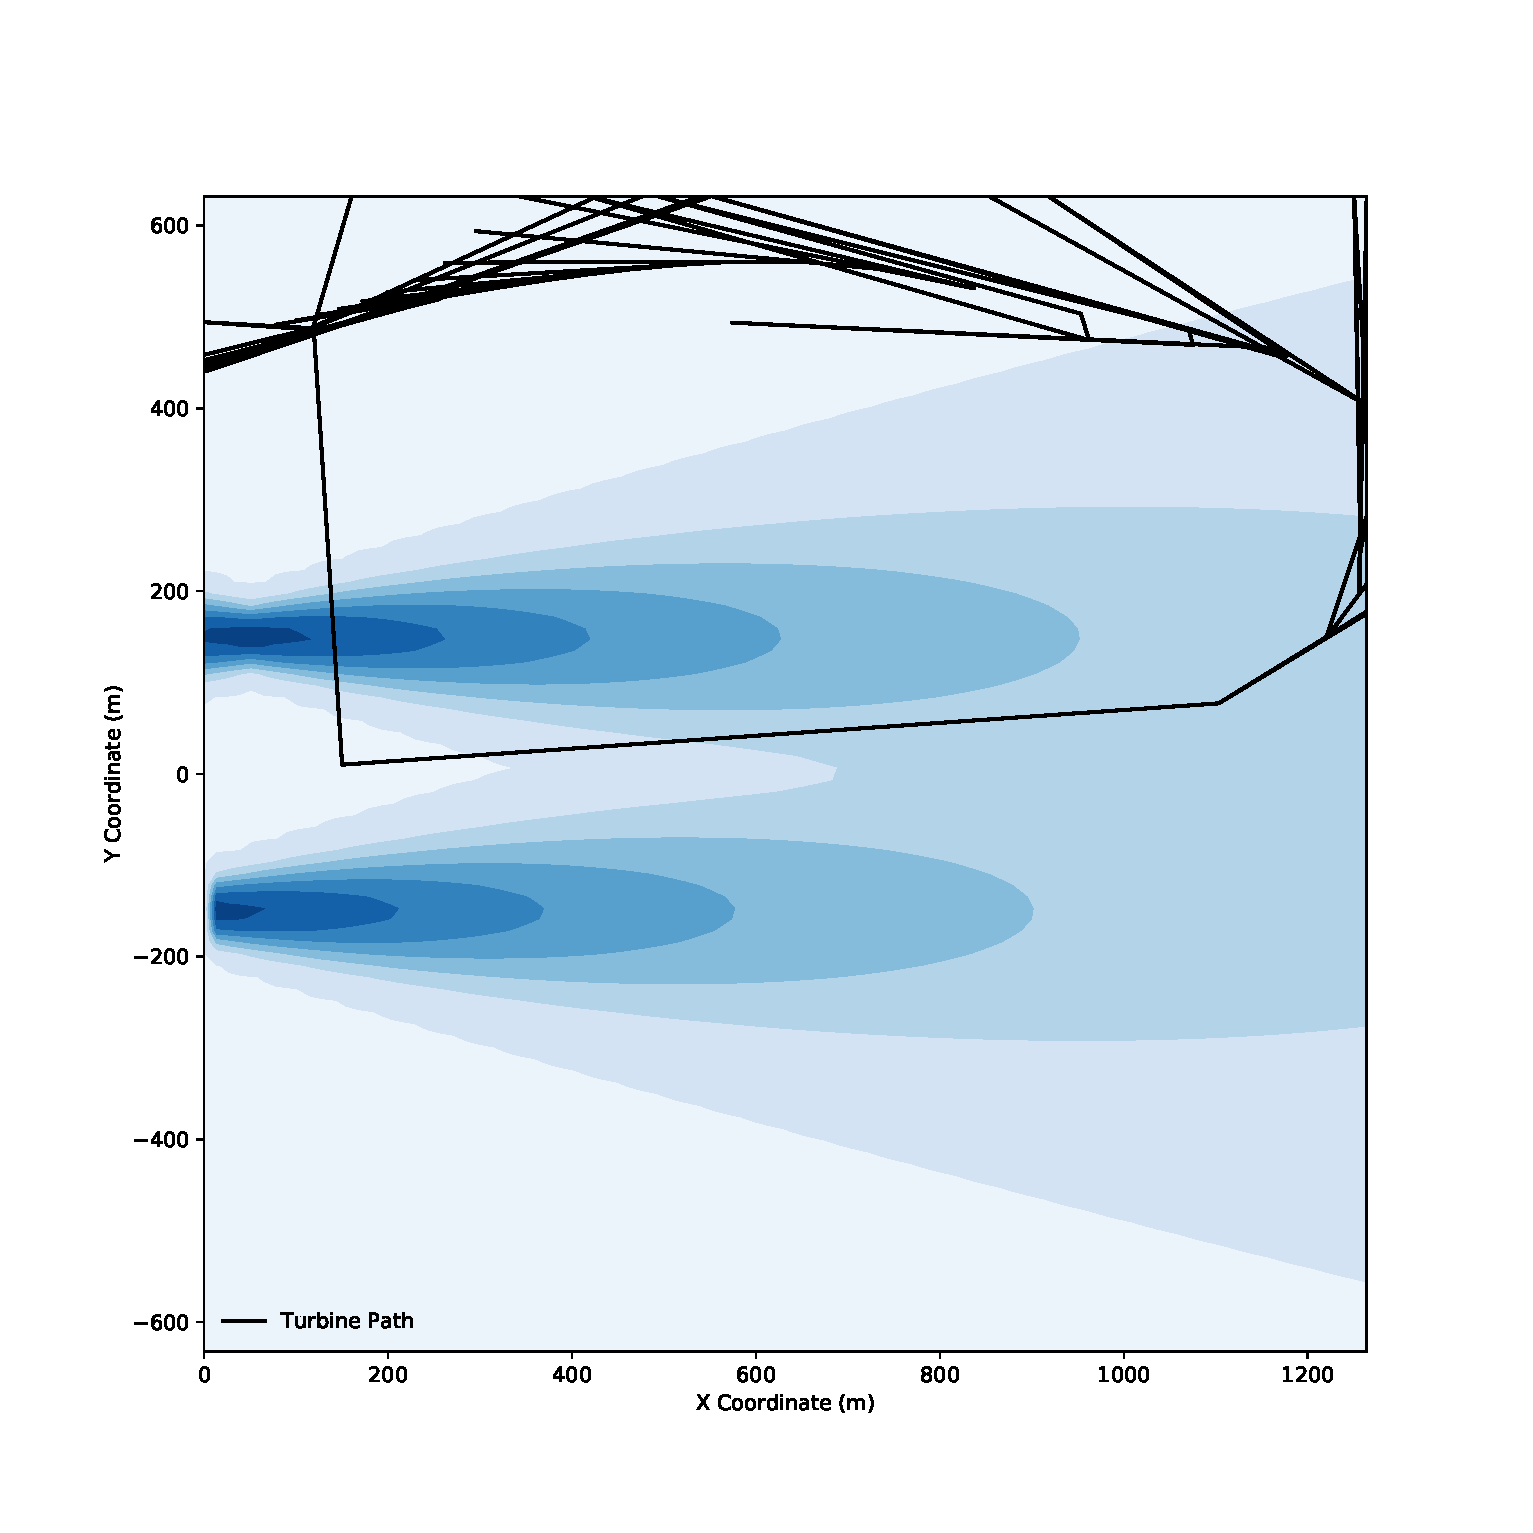
\includegraphics[width=0.35\textwidth]{SmallScaleJensenWECGraphContour}
    }
    \subfigure[]{
        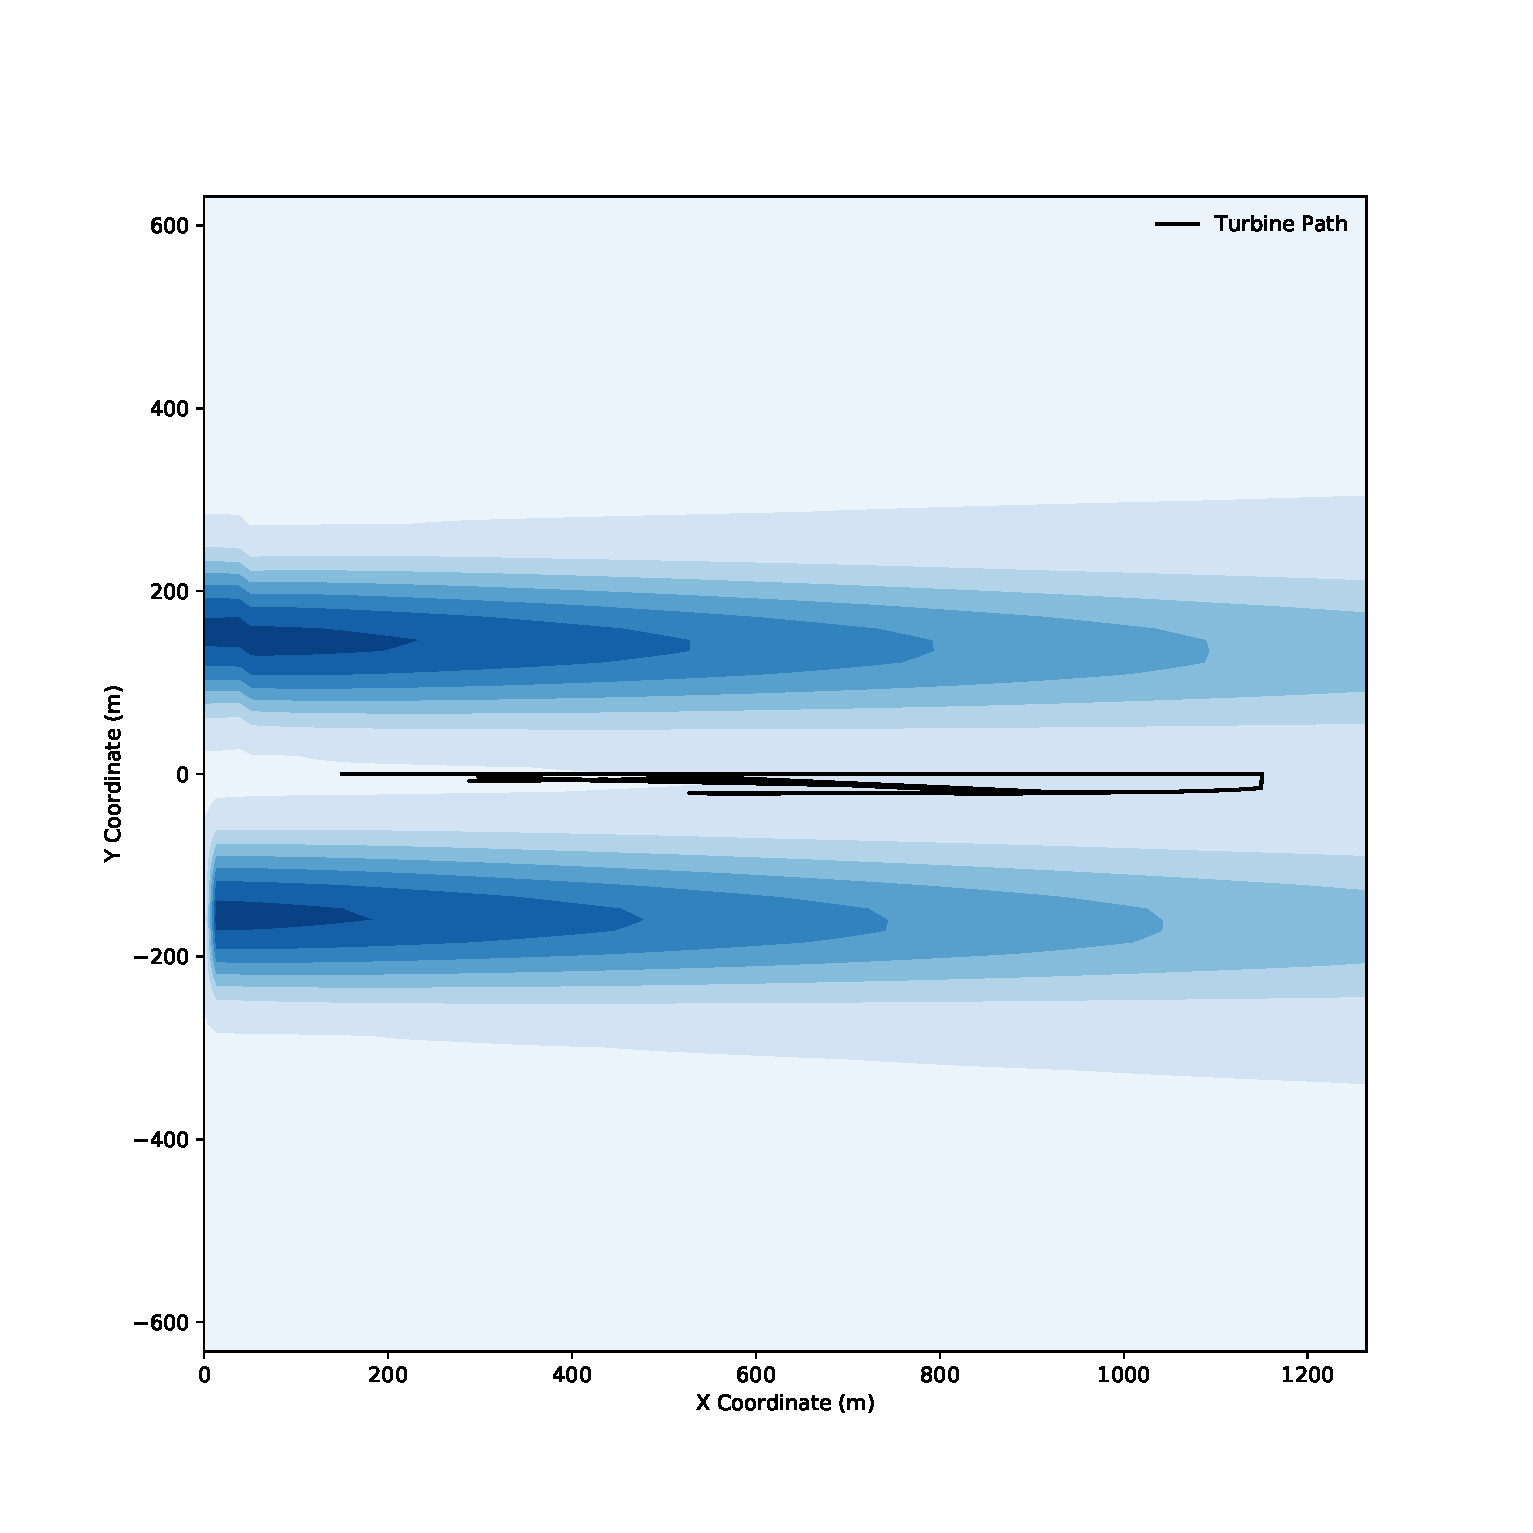
\includegraphics[width=0.35\textwidth]{SmallScaleFLORISSENonWECGraphContour}
    }
    \subfigure[]{
        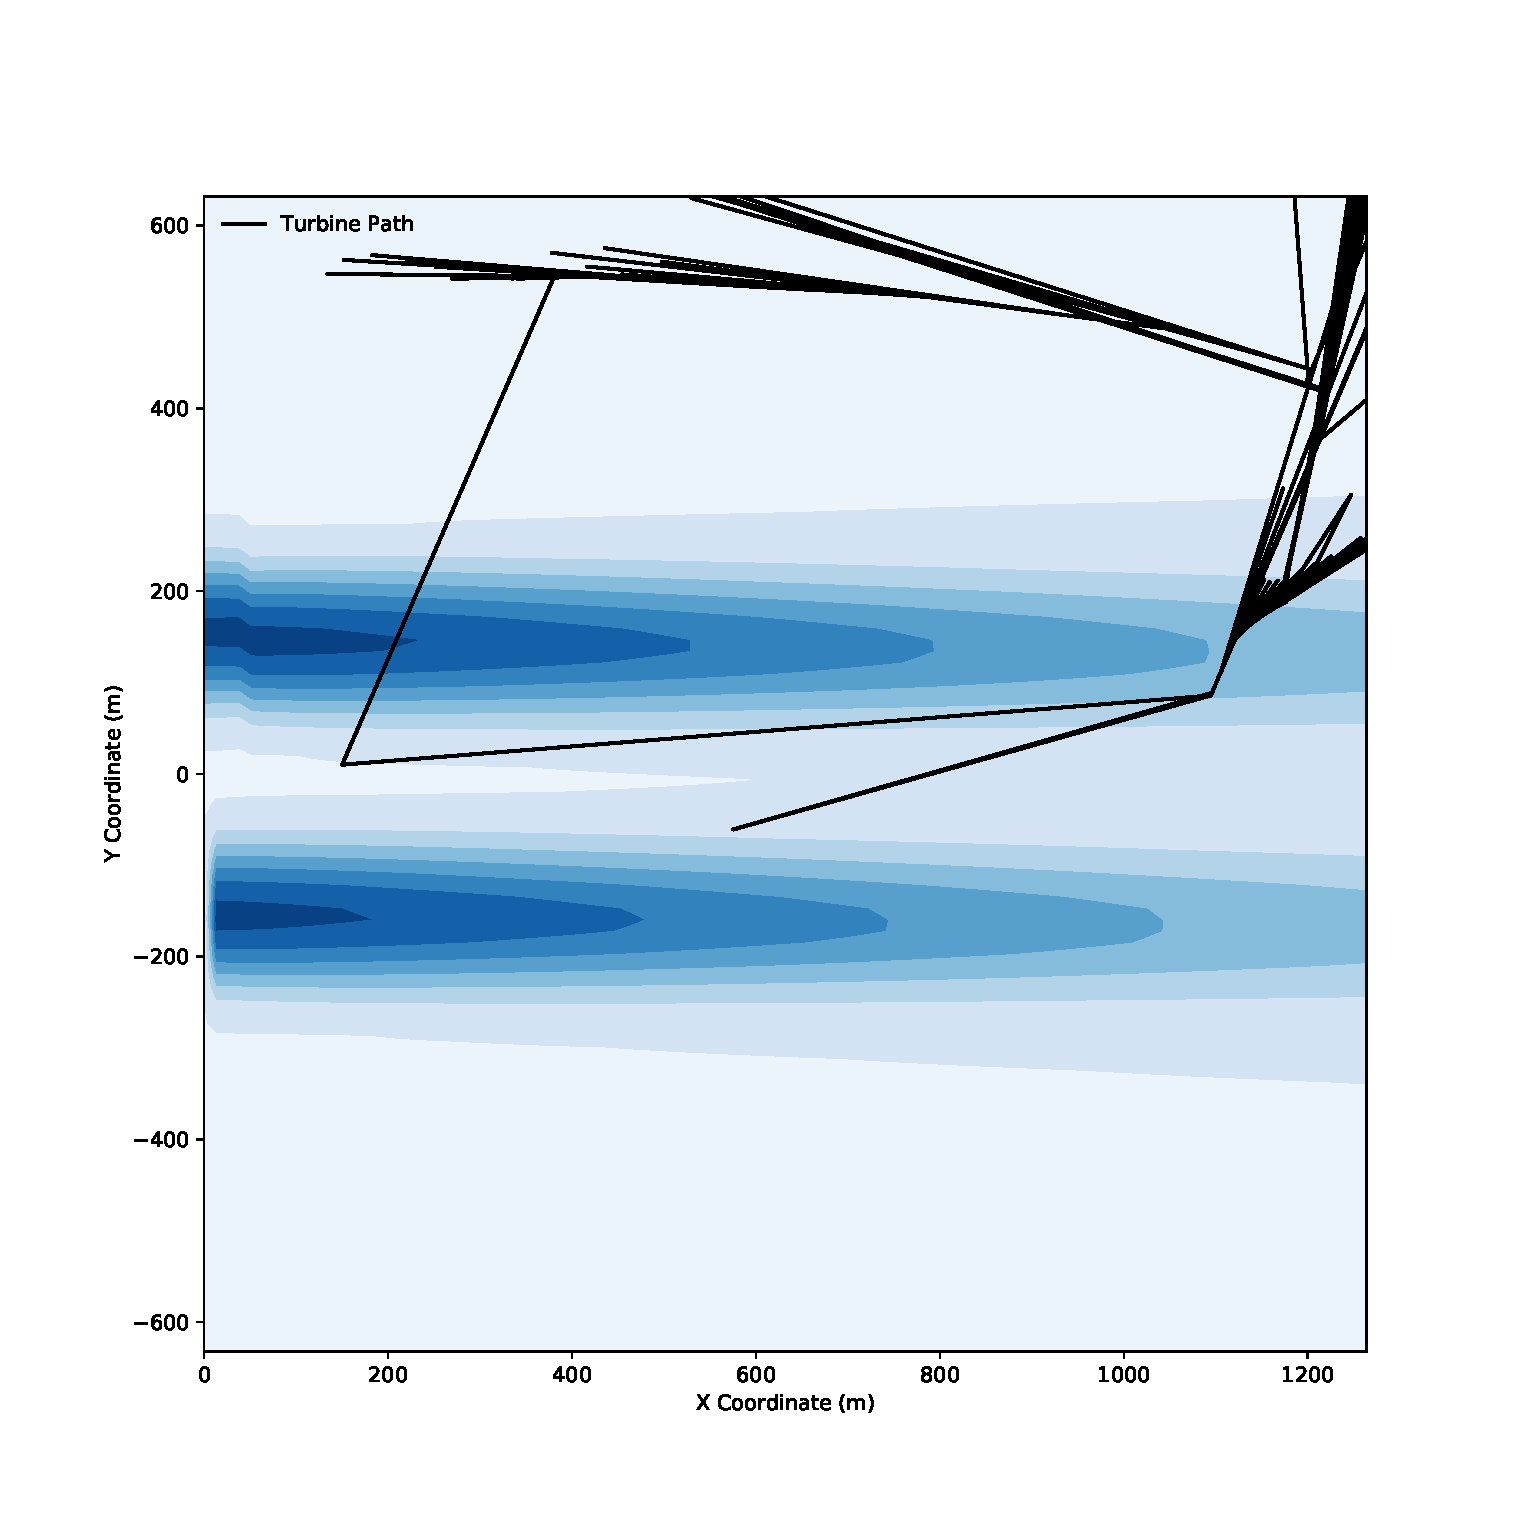
\includegraphics[width=0.35\textwidth]{SmallScaleFLORISSEWECGraphContour2}
    }
    \subfigure[]{
        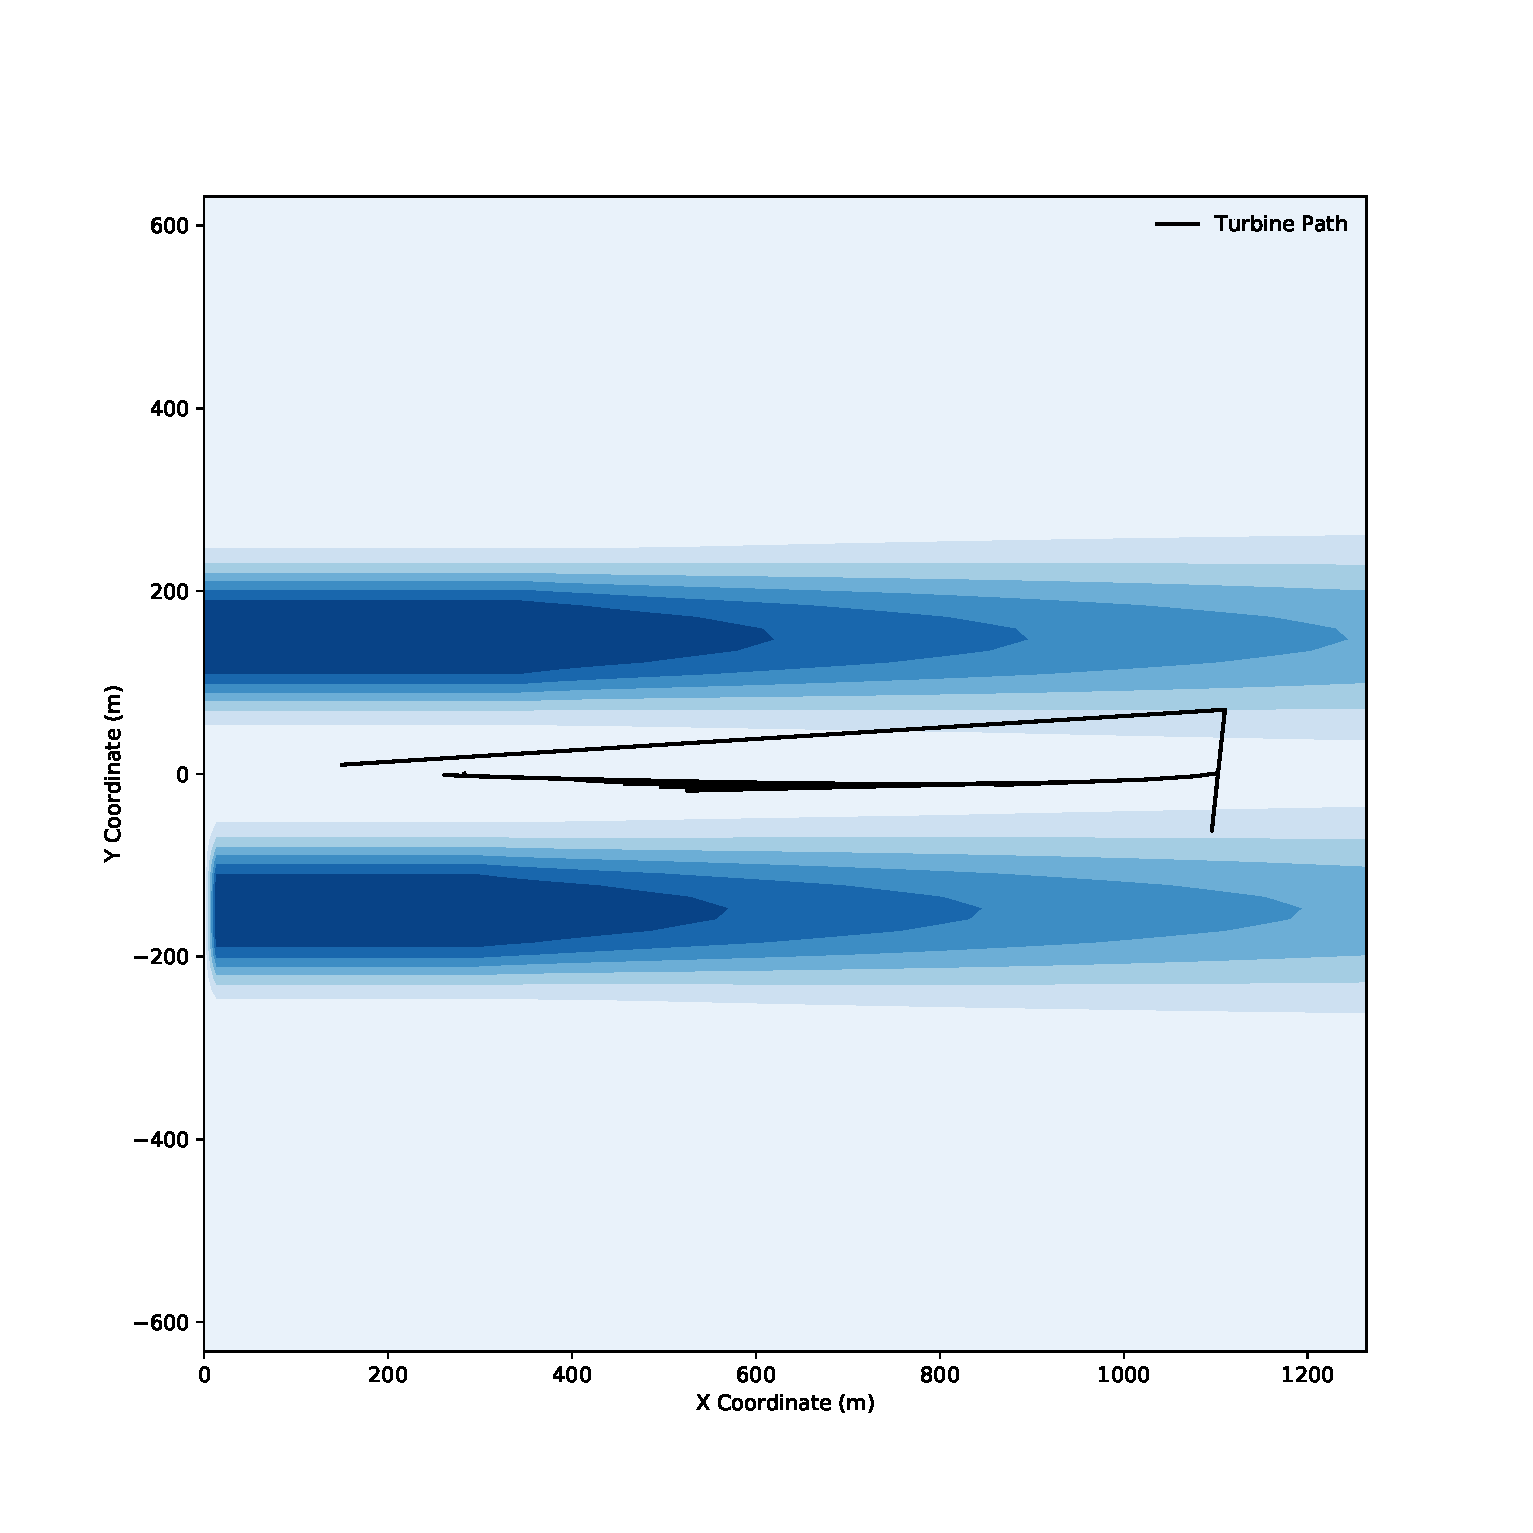
\includegraphics[width=0.35\textwidth]{SmallScaleBPANonWECGraphContour}
    }
    \subfigure[]{
        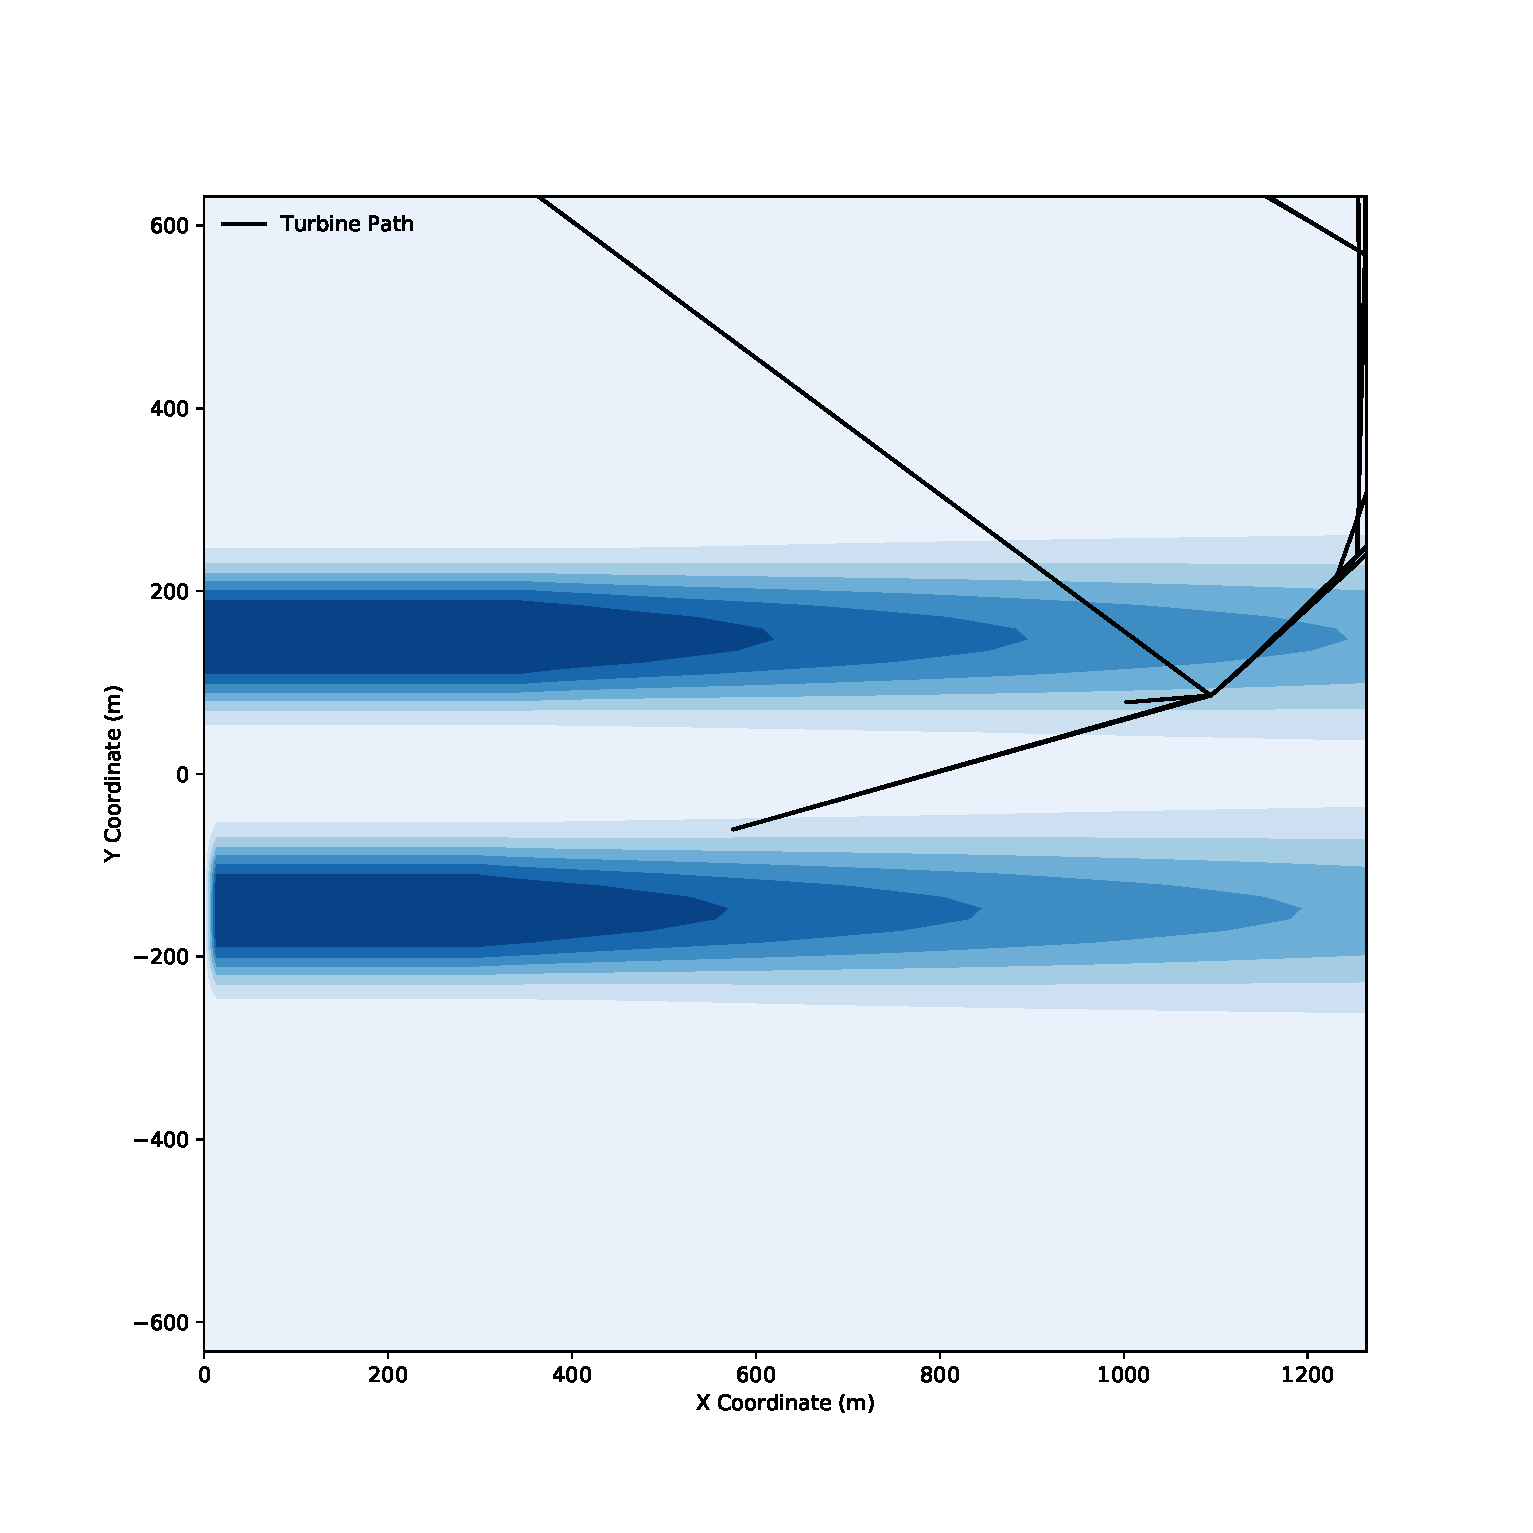
\includegraphics[width=0.35\textwidth]{SmallScaleBPAWECGraphContour}
    }
    \caption{Small-scale optimization contour plots with eastward flowing wind, two stationary upwind turbines, and one variable downwind turbine. Optimizations are shown without WEC (left) and with WEC (right). Each row represents a different turbine wake model: Jensen Cosine, FLORIS, and BPA, respectively.}
    \label{fig:SmallScaleOptimizations}
\end{figure}

%\subsection{Case 0.75 Results}
%Results for large-scale optimizations for all wake models? Don't have the FLORISSE results since I haven't had time to fix the tapenade gradient code, although I could run the model with the finite-difference gradient code.

\subsection{Case 1 Results}
Results for case 1 are presented in \cref{fig:aep1,fig:fcalls1,tab:case1}. The SNOPT results had the lowest mean AEP (167.39 GWh) and the highest standard deviation (2.74 GWh). The results using WEC with SNOPT had a mean AEP and standard deviation of 174.13 GWh and 2.26 GWh respectively. The results using NSGA-II had the highest mean AEP (175.98 GWh) and lowest standard deviation (0.65 GWh) of the optimization methods tested. The maximum AEP values for SNOPT, SNOPT with WEC, and NSGA-II were 174.23 GWh, 177.25 GWh, and 177.69 GWh respectively (see \cref{tab:case1}). The AEP results for all cases were fairly normally distributed, but the results with SNOPT and WEC had several low outliers (see \cref{fig:aep1}).

 The median number of function calls required by SNOPT, SNOPT with WEC, and NSGA-II were 246, 1,026, and 368,003 respectively. The high values for function calls required by SNOPT, SNOPT with WEC, and NSGA-II were 10,461, 11,216, and 1,342,723 respectively. However, the function call distributions for both SNOPT and SNOPT with WEC are highly skewed, with more runs grouped at the low end of the distributions. The function call distribution for NSGA-II is more normally distributed, but is still slightly skewed (see \cref{fig:fcalls1}).

\begin{figure}[h!]  
\centering
\begin{minipage}[t]{18pc}    
\centering
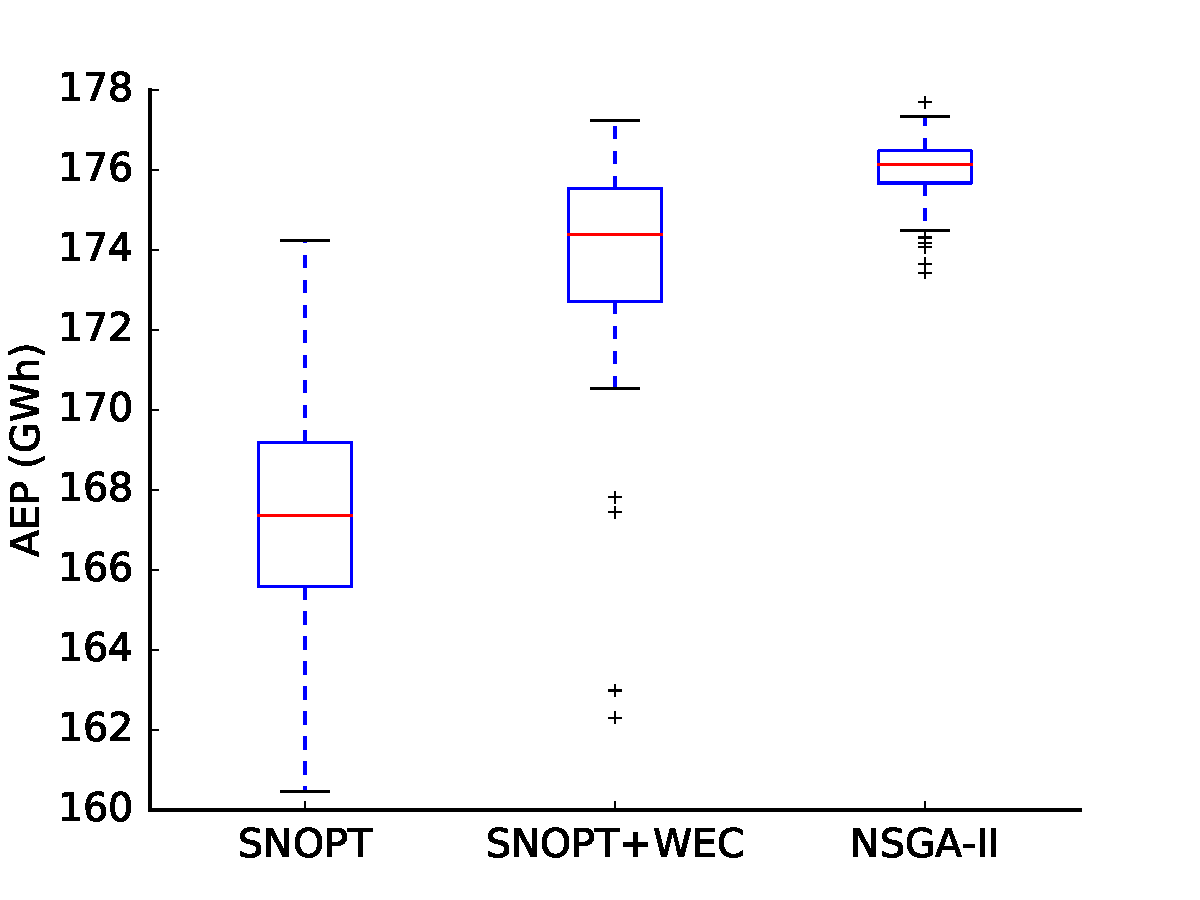
\includegraphics[width=\textwidth, trim={0cm 0cm 0cm 0cm}]{16turbs_results_aep}
\caption{Box plot comparing the AEP results across each optimization approach for case 1 (16     turbines).}
\label{fig:aep1}
\end{minipage}\hspace{1pc}
\begin{minipage}[t]{18pc}    
\centering
\def\big{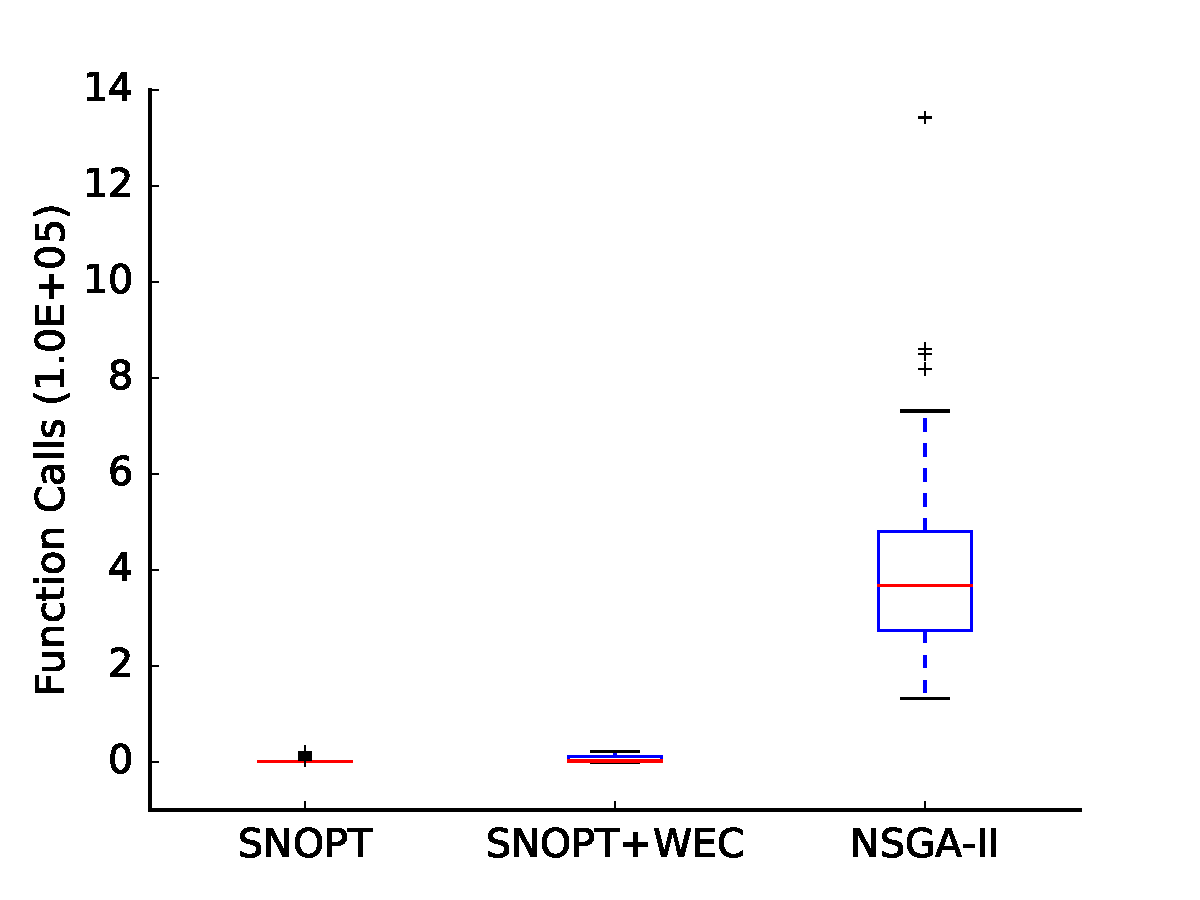
\includegraphics[width=\textwidth]{16turbs_results_fcalls}}
\def\little{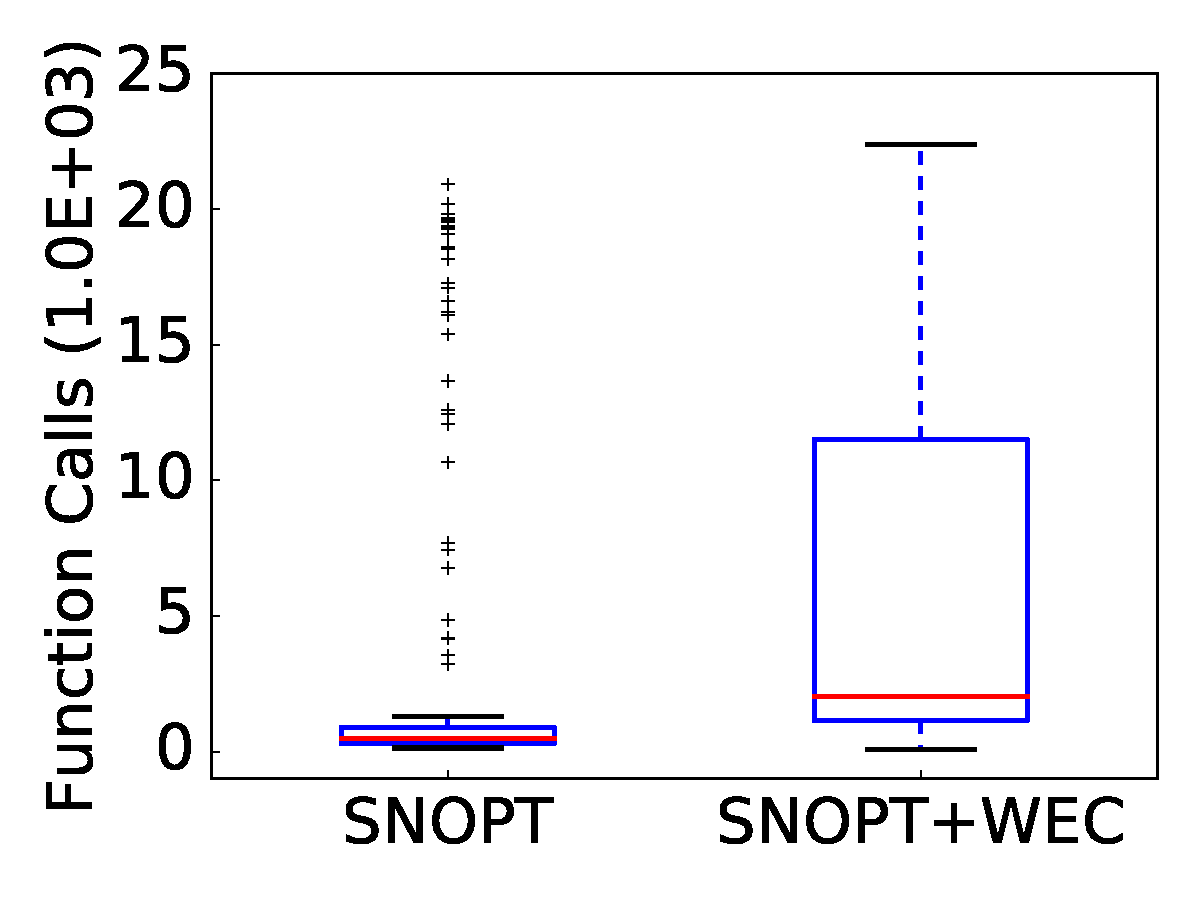
\includegraphics[width=0.5\textwidth]{16turbs_results_fcalls_snopt}}
\def\stackalignment{l}
\topinset{\little}{\big}{1cm}{1.25cm}

\caption{Box plot comparing the number of function calls used by each optimization approach for case 1 (16 turbines).}
\label{fig:fcalls1}
\end{minipage}
\end{figure}
%

\subsection{Case 2 Results}

Results for case 2 are presented in \cref{fig:aep2,fig:fcalls2,tab:case2}. The NSGA-II results had the lowest mean AEP for case 2 (331.98 GWh) and the second highest standard deviation (3.74 GWh). The results using WEC with SNOPT had the highest mean AEP and lowest standard deviation, 379.94 GWh and 2.24 GWh respectively. The results using SNOPT by itself had the second highest mean AEP (364.93 GWh), but highest standard deviation (5.88 GWh) of the optimization methods tested. The maximum AEP values for SNOPT, SNOPT with WEC, and NSGA-II were 380.71 GWh, 384.55 GWh, and 342.56 GWh respectively (see \cref{tab:case2}). The AEP results for all cases were fairly normally distributed, but the results with SNOPT alone had several low outliers (see \cref{fig:aep1}).

 The median number of function calls required by SNOPT, SNOPT with WEC, and NSGA-II were 242.5, 1,482, and 551,003 respectively. The high values for function calls required by SNOPT, SNOPT with WEC, and NSGA-II were 893, 6,748, and 1,368,003 respectively. However, the function call distributions for SNOPT with WEC was again highly skewed, with more runs grouped at the low end of the distribution with quite a few outliers at the higher end. The function call distributions for NSGA-II and SNOPT and are more normally distributed, but are also slightly skewed (see \cref{fig:fcalls1}).

It may be noted that the function calls required for each method to solve case 2 are comparable to the function calls required for case 1. This is likely due to a combination of design variable and constraint scaling difference, the objective being scaled down more for case 2 ($1\times10^{-5}$) than for case 1 ($1\times10^{-3}$), and the SNOPT objective tolerance being loosened from case 1 ($1\times10^{-5}$) to case 2 ($1\times10^{-4}$) because the higher tolerance is difficult to reach for larger problems.

\begin{figure}[ht]
\centering
\begin{minipage}[t]{18pc}
\centering
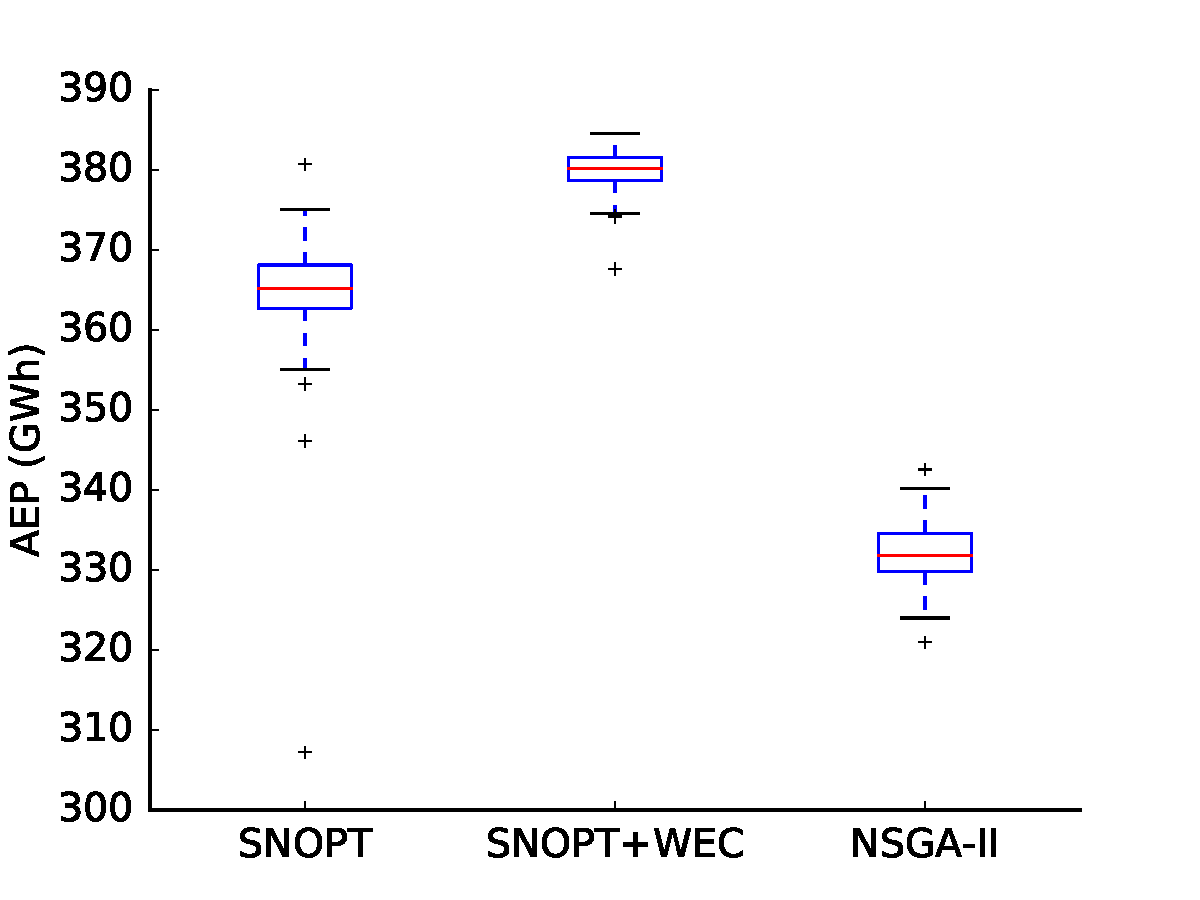
\includegraphics[width=\textwidth, trim={0cm 0cm 0cm 0cm}]{38turbs_results_aep}
\caption{Box plot comparing the AEP results across each optimization approach for case 2 (38 turbines).}
\label{fig:aep2}
\end{minipage}\hspace{1pc}%
\begin{minipage}[t]{18pc}
\centering
\def\big{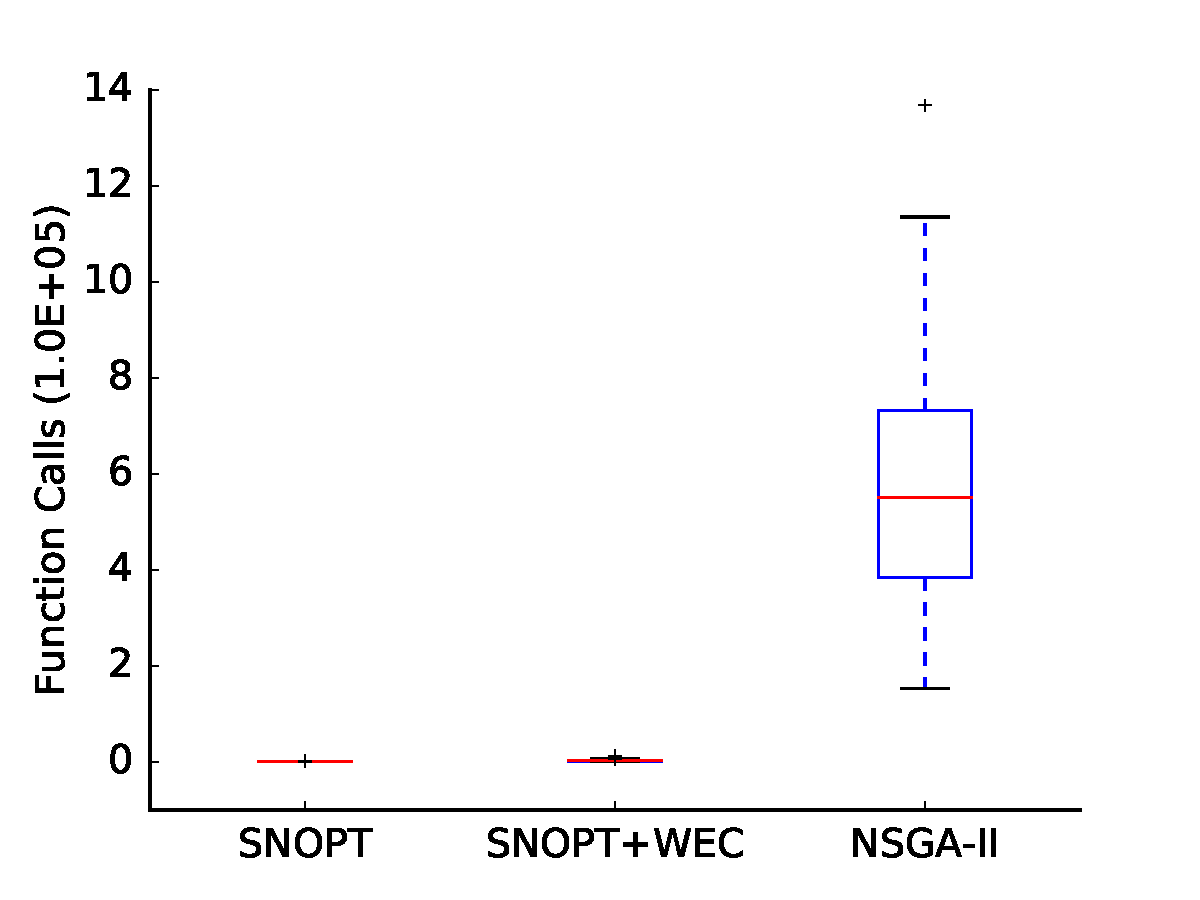
\includegraphics[width=\textwidth]{38turbs_results_fcalls}}
\def\little{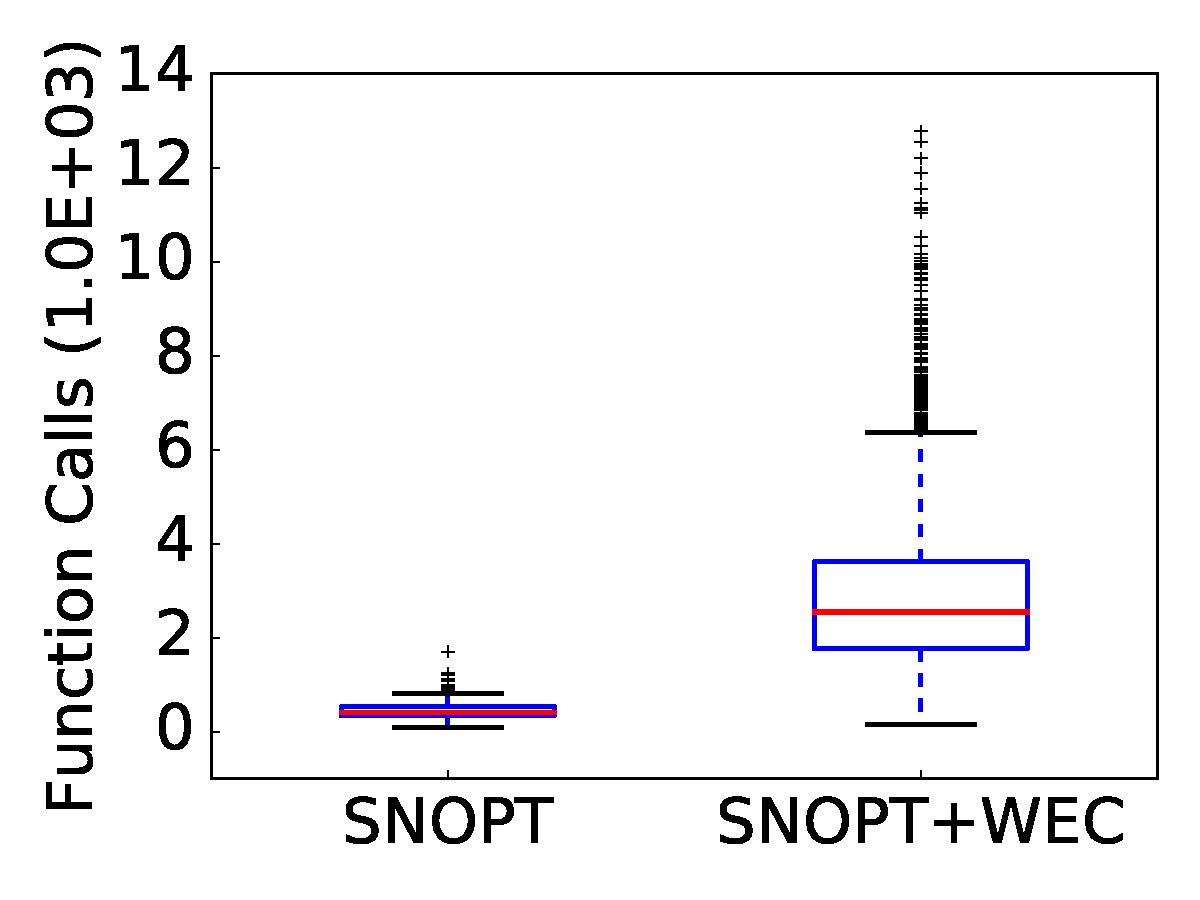
\includegraphics[width=0.5\textwidth]{38turbs_results_fcalls_snopt}}
\def\stackalignment{l}
\topinset{\little}{\big}{1cm}{1.25cm}
  
\caption{Box plot comparing the number of function calls used by each optimization approach for case 2 (38 turbines).}
\label{fig:fcalls2}
\end{minipage} 
\end{figure}
%
\begin{table}
  \caption{Optimization Results for Case 1}
  \label{tab:case1}
  \centering
  \begin{tabular}{lcrrrcrrrrr}
  \br
   & & \multicolumn{3}{c}{Function Calls} &  & \multicolumn{5}{c}{Annual Energy Production (GWh) } \\
   \cline{3-5}\cline{7-11}
  Method  & & Median & Low & High & & Mean & SD & Low & High\\
   \cline{1-1}\cline{3-5}\cline{7-11}
  SNOPT  & & 246 & 67 & 10,461 & & 167.39 & 2.74 & 160.45 & 174.23   \\
  SNOPT+WEC & & 2,462.5 & 612 & 22,394 &  &  174.13 & 2.26 & 162.31 & 177.25 \\
  NSGA-II & & 368,003 & 131,843 & 1,342,723 & & 175.98 & 0.65 & 173.44 & 177.69\\
  \br
  \multicolumn{11}{p{0.7\textwidth}}{Note: AEP for the layout in \cref{fig:grid_case} was 160.18 GWh} 
  \end{tabular}
\end{table}

\begin{table}
  \caption{Optimization Results for Case 2}
  \label{tab:case2}
  \centering
  \begin{tabular}{lcrrrcrrrrr}
  \br
   & & \multicolumn{3}{c}{Function Calls} &  & \multicolumn{5}{c}{Annual Energy Production (GWh) } \\
   \cline{3-5}\cline{7-11}
  Method  & & Med. & Low & High & & Mean & SD & Low & High\\
   \cline{1-1}\cline{3-5}\cline{7-11}
  SNOPT  & & 242.5 & 82 & 893 & & 364.93 & 5.88 & 307.21 & 380.71   \\
  SNOPT+WEC & & 4,151 & 2,004 & 13,496 &  &  379.94 & 2.24 & 367.63 & 384.55 \\
  NSGA-II & & 4,342,643 & 913,523 & 8,949,763 & & 355.23 & 1.93 & 346.90 & 359.66\\
  \br
  \multicolumn{11}{p{0.7\textwidth}}{Note: AEP for the layout in \cref{fig:round_case} was 352.02 GWh} 
  \end{tabular}
\end{table}

\section{Discussion}
In the WFLO problem, we are looking for high AEP values, a tight distribution, and relatively few function calls. The benefit of high AEP means that the resulting wind farm will be more efficient, likely leading to a reduced cost of energy. A tight distribution means that the method is consistent, that the optimized solution is independent of the starting layout. The tighter the distribution the fewer optimizations need to be run before we are confident that we have one of the best wind farm designs we can get. A low number of function calls means that wind farm design can be done more cheaply and that more variables could potentially be tested, which could again lead to a lower cost of energy. Each of the methods tested demonstrated at least one of these characteristics.

The results from case 0 appear promising (\cref{fig:SmallScaleOptimizations}). Whereas optimizations without WEC are unable to escape the local optimum between wakes, optimizations with WEC are able to escape the local optimum and achieve better optima. These  results suggest that large-scale optimization test results should display similar improvements in optimization performance.

The relatively high AEP results from NSGA-II on the smaller case, compared to the relatively low AEP results of NSGA-II on larger case illustrates an inherent weakness of gradient-free algorithms. Namely, that increased dimensionality generally leads to a decrease in the performance of gradient-free algorithms \cite{rios2013-grad-free-comparison}. As shown by the high number of function calls for NSGA-II, gradient-free algorithms also tend to take a relatively long time to run. These weakness are the main drivers for increasing interest in gradient-based algorithms.

The relatively wide spread and moderate results from SNOPT on both cases demonstrate one of the weaknesses of gradient-based algorithms. While gradient-based algorithms tend to need fewer function calls, and thus typically less time, they are highly susceptible to local optima. That WEC AEP results were relatively much higher and less spread for both test cases, as compared with SNOPT, seems to indicate that the process is at least partially remedying the problem of local optima.

The high values of AEP and lower standard deviation of AEP compared to SNOPT with WEC, indicates that SNOPT with WEC is more accurate and reliable. So much so that, ignoring outliers, the probability distributions for SNOPT with and without WEC from case 2 just overlap only slightly (see \cref{fig:aep2}). This reliability does come at the cost of more function calls than SNOPT without WEC. The increase in function calls when using WEC is expected because the relaxation optimization method ran nine optimizations to convergence (one for each value of $\xi$) for every one optimization by SNOPT alone. The number of function calls needed for WEC was still only a fraction of what was need for NSGA-II, so the added cost in function calls seems reasonable from that perspective. However, because WEC has a smaller probability distribution than SNOPT by itself, fewer runs would be needed to gain the same level of confidence in the results. The reduction in overall runs could mean an overall reduction in the number of function evaluations for WEC as compared to SNOPT alone.

\section{Conclusion}
The WEC proposed in this paper uses characteristics of typical wake models to reduce the multi-modal nature of the design space. We tested WEC on two WFLO problems, one with 16 turbines and one with 38 turbines. Results using WEC show a $4\%$ mean optimized AEP improvement compared to gradient-based optimization without WEC for both test cases. A gradient-free algorithm had a mean optimized AEP that was $1\%$ higher than WEC for the 16-turbine case, but WEC resulted in a $10\%$ higher mean optimized AEP compared to a gradient-free optimization method for the 38-turbine problem.

\todo{Jared: what do you think of this paragraph?}
Applying WEC to other turbine wake models (e.g., Jensen Cosine and FLORIS) produced mixed results. Small-scale optimization tests resulted in promising results that seemed to predict desirable performance in large-scale optimizations. However, the large-scale optimizations did not return similarly promising results, and seemed to indicate even undesirable results. Further work will be necessary to determine the root cause of these unexpected issues.

%Future work should investigate potential improvements and best practices for WEC, apply WEC to other wake models, provide a more complete comparison to gradient-free wind farm layout optimization including discrete parameterization, and validate the results obtained through WEC using a higher-order modeling approach such as Large Eddy Simulation (LES).

Future work should investigate potential improvements and best practices for WEC, provide a more complete comparison to gradient-free wind farm layout optimization including discrete parameterization, and validate the results obtained through WEC using a higher-order modeling approach such as Large Eddy Simulation (LES).

\ack 
This work was supported by the National Science Foundation under Grant No. 1539384. Any opinions, findings, and conclusions or recommendations expressed in this material are those of the authors and do not necessarily reflect the views of the National Science Foundation.

\section*{References}
\bibliographystyle{iopart-num}
\bibliography{references/all_refs}

\end{document}

